% ============================================================
% ContextForge v2.3 — Architecture-First Persistent Agentic
% Memory via Model Context Protocol
%
% Author : Trilochan Sharma (Independent Researcher)
% Email  : parnishklpo@gmail.com
% Date   : April 2026
% Version: 2.3  (v3 OR-gate security numbers; Suite 15 v2 with
%                recency-weighted retrieval; Fig 19 security
%                trade-off scatter; honest Phi/CSS update)
%
% HOW TO COMPILE (Overleaf or local):
%   pdflatex contextforge_v2_final
%   bibtex   contextforge_v2_final
%   pdflatex contextforge_v2_final
%   pdflatex contextforge_v2_final
%
% FIGURES REQUIRED (upload to figures/ subfolder):
%   Core architecture figures (generate with python research/figures/gen_all.py):
%     figures/fig_system_architecture.png
%     figures/fig_mcp_dataflow.png
%     figures/fig_entropy_gate.png
%     figures/fig_voh_tiers.png
%     figures/fig_temporal_correlator.png
%     figures/fig_calibration_sweep.png
%     figures/fig_token_savings.png
%     figures/fig_ablation.png
%     figures/fig_radar.png
%     figures/fig_crdt_convergence.png
%     figures/fig_perplexity_gate.png
%     figures/fig_weight_sensitivity.png
%   Suite 14 FPR-fix figures (generate with python research/figures/gen_fpr_fix_figures.py):
%     figures/output/figure_13_mode_comparison.png
%     figures/output/figure_14_entropy_distributions_v2.png
%     figures/output/figure_15_edge_trigger_breakdown.png
%   Suite 15 v2 memory quality figures (generate with
%     python benchmark/benchmark_memory/figures/gen_memory_figures_v2.py):
%     figures/output/fig_16_memory_radar_v2.png
%     figures/output/fig_17_memory_bars_v2.png
%     figures/output/fig_18_memory_heatmap_v2.png
%   Security trade-off scatter (generate with
%     python research/figures/gen_security_tradeoff_fig19.py):
%     figures/output/fig_19_security_tradeoff.png
% ============================================================

\documentclass[11pt,twocolumn]{article}

% ── Packages ──────────────────────────────────────────────────────────────────
\usepackage[top=1in,bottom=1in,left=0.75in,right=0.75in]{geometry}
\usepackage{authblk}
\usepackage{amsmath}
\usepackage{amssymb}
\usepackage{graphicx}
\usepackage{booktabs}
\usepackage{tabularx}
\usepackage{multirow}
\usepackage{array}
\usepackage[numbers,sort&compress]{natbib}
\usepackage[colorlinks=true,linkcolor=blue!70!black,
            citecolor=blue!70!black,urlcolor=blue!70!black]{hyperref}
\usepackage{xcolor}
\usepackage{microtype}
\usepackage{float}
\usepackage{caption}
\usepackage{enumitem}
\usepackage{balance}

% ── Figure path ───────────────────────────────────────────────────────────────
\graphicspath{{figures/}{figures/output/}}

% ── Caption style ─────────────────────────────────────────────────────────────
\captionsetup{font=small,labelfont=bf}

% ── Column separation ─────────────────────────────────────────────────────────
\setlength{\columnsep}{18pt}

% ── Title ─────────────────────────────────────────────────────────────────────
\title{%
  \textbf{ContextForge: Architecture-First Persistent Agentic Memory\\
    via Model Context Protocol}\\[0.35em]
  \large\textit{Multi-Trigger OR-Gate Security, OR-Set CRDT Sync,
    Tri-Core Failover,\\
    Differential Context Injection, Recency-Weighted Retrieval,
    and a Memory Quality Benchmark}%
}

\author[1]{Trilochan Sharma}
\affil[1]{Independent Researcher \quad \texttt{parnishklpo@gmail.com}}

\date{April 2026}

% =============================================================================
\begin{document}
\maketitle

% ── Abstract ──────────────────────────────────────────────────────────────────
\begin{abstract}
Stateless Retrieval-Augmented Generation (RAG) systems suffer from three
structural failure modes: zero adversarial block rate, high cold-start
failover latency (${\sim}480$\,ms), and unbounded context injection that
grows linearly with session history.
We present \textbf{ContextForge}, a five-pillar agentic memory architecture
that simultaneously addresses all three failures and exposes every capability
as a \textbf{22-tool Model Context Protocol (MCP)} server---providing
persistent, adversarially-hardened memory in Claude Desktop, Cursor,
VS Code, and Windsurf with zero client-side code changes.

The write-security backbone is \texttt{ReviewerGuard}, an append-only SQLite
event ledger with a \emph{multi-trigger OR-gate} (v3): Path~A fires on
char-level Shannon entropy ($H_{\mathrm{char}} \geq H^{*} = 4.8$\,bits/char,
catching obfuscated/encoded payloads); Path~B fires on injection intent score
($\geq 0.70$ over 22 patterns + charter-keyword overlap, catching natural-language
injections); Path~C (trigram perplexity gate, $P^{*}=231.8$) provides orthogonal
defence against entropy-mimicry.  Any single path independently blocks the write.
Verified-origin traffic receives an elevated threshold ($H^{*}_{\mathrm{VOH}} =
4.375$\,bits via HMAC-SHA256) and a Sliding-Window Temporal Correlator detects
slow-drip multi-write escalation sequences at 100\% detection, 0\% FPR.

An OR-Set CRDT synchronisation layer (\texttt{src/sync/crdt\_sync.py})
supports conflict-free concurrent writes from multiple IDE clients with
add-wins semantics, verified at 100\% convergence across three concurrent-write
scenarios including a full split-brain reconnection.

\textbf{Suite 14 results (300 samples, measured).}
In \texttt{CF\_MODE=experiment} (v3 multi-trigger OR-gate):
benign FPR\,=\,1\% (vs.\ 96\% in PAPER mode, $\Delta=-95$\,pp),
adversarial recall\,=\,55\% (vs.\ 95\% in PAPER mode; the tradeoff is
deliberate---Path~A replaces the miscalibrated word-level $H^{*}\!=\!3.5$ gate
that produced 96\% benign FPR), edge-case FPR\,=\,16\% ($\Delta=-81$\,pp).
The 45\% adversarial miss rate is confined to paraphrased natural-language
injections with max intent\_score\,=\,0.50, identified as the primary target
for Path~C (perplexity gate).  Hardened-RAG achieves 71\% recall at 45\%
edge FPR---higher recall but substantially worse precision on maintenance text.

\textbf{Suite 15 v2 results (160 samples, 6 systems, measured).}
A Memory Quality Benchmark evaluates retrieval recall, update preference,
delete fidelity, and poison resistance using a zero-LLM harness with BM25
retrieval and the REAL ReviewerGuard v3 gate.
Version~2 adds recency-weighted retrieval
($\exp(-\lambda\Delta t)$, $\lambda=0.0001$\,s$^{-1}$),
raising update accuracy from 0.229 to 0.600 ($+37.1$\,pp) at a $-13.4$\,pp
cost in Recall@3 (0.967\,$\to$\,0.833).
ContextForge achieves a Memory Integrity Score (MIS) of \textbf{0.801}
(Recall@3\,=\,0.833, Update\,=\,0.600, Delete\,=\,1.000, Poison\,=\,0.771),
ranking \emph{first} among six systems.
HardenedRAG is second at MIS\,=\,0.753 ($\Delta=-4.8$\,pp);
unguarded systems score MIS\,$\leq$\,0.595 with zero poison resistance.

Across 990 benchmark tests total, additional highlights include:
$-68.9\%$ failover latency, $+70.2$\,pp token noise reduction, Weighted
Safety Index $\Phi = 62.2\%$ (v3 EXPERIMENT mode), CRDT convergence rate\,=\,1.0,
and external macro-F1\,=\,0.755 on \texttt{deepset/prompt-injections} ($n=116$).
\end{abstract}

% =============================================================================
\section{Introduction}
\label{sec:intro}

Modern AI coding workflows rely on Retrieval-Augmented Generation~\cite{lewis2020rag}
to supply context from external knowledge stores. While RAG substantially improves
factual grounding~\cite{gao2023retrieval}, dominant implementations share a
critical architectural weakness: they are \emph{stateless}. Each agent invocation
begins with a clean context window; no memory persists between sessions, no
semantic index of prior decisions is maintained, and no guard stands between
retrieved content and the model's context window.

This statelessness produces three measurable failure modes.

\textbf{FM-1: Adversarial injection.}
Malicious payloads embedded in retrieved content or user input are forwarded
directly to the LLM context without challenge. All four baseline systems
(StatelessRAG, MemGPT-style, LangChain-Buffer) report 0\% adversarial block
rate; even Hardened-RAG's keyword-only filter reaches only 71\% ABR against
obfuscated payloads.

\textbf{FM-2: High failover latency.}
When the primary LLM provider trips its rate limit or goes offline, naive
sequential failover introduces ${\sim}480$\,ms of dead time---breaking the
interactive feel of an IDE session.

\textbf{FM-3: Unconstrained context injection.}
Without a budget gate, context size grows with corpus size. At 200 stored
decisions, a ``paste-all'' CLAUDE.md approach injects 30{,}000 tokens per
session; LangChain-Buffer's naive left-truncation injects $1{,}590 \pm 11$
tokens per query---all unfiltered. This grows without bound and eventually
collapses within the model's context window.

ContextForge addresses all three failure modes through a five-pillar
architecture (Section~\ref{sec:architecture}) exposed as a 22-tool MCP server
(Section~\ref{sec:mcp}). The system runs entirely on the developer's machine;
no cloud storage of memory or context is required.

\subsection*{Contributions}

\begin{itemize}[leftmargin=*,topsep=2pt,itemsep=2pt]
  \item A five-pillar agentic memory architecture (Transport, Router, Memory,
    Retrieval, Sync) that closes FM-1 through FM-3 simultaneously.
  \item \textbf{ReviewerGuard v3 multi-trigger OR-gate}: an append-only
    write ledger combining char-level entropy (Path~A), injection intent scoring
    over 22 patterns (Path~B), and trigram perplexity anomaly detection (Path~C)
    as independently sufficient blocking conditions. Suite~14 (300 samples)
    measures benign FPR\,=\,1\%, adversarial recall\,=\,55\%, edge-case
    FPR\,=\,16\% vs.\ PAPER mode's 96\%/95\%/97\%---a 95\,pp FPR reduction
    with an accepted 40\,pp recall tradeoff on paraphrased injections.
  \item A Sliding-Window Temporal Correlator detecting slow-drip escalation
    sequences (100\% detection, 0\% FP at $\nabla^{*}\!=\!0.15$\,bits/write)
    with structural robustness: ${\approx}60\%$ of near-threshold evasion
    attempts overshoot the gradient threshold by construction.
  \item Tiered Clearance Logic (VOH) with HMAC-SHA256 tokens
    ($H^{*}_{\mathrm{VOH}} = 4.375$\,bits) for high-entropy internal traffic.
  \item A trigram perplexity gate (Pass~0.5, $P^{*}=231.8$) with zero external
    dependencies, catching entropy-mimicry payloads scoring $>2\times P^{*}$.
  \item An OR-Set CRDT synchronisation layer with vector-clock causal ordering
    and add-wins semantics, verified at 100\% convergence across
    concurrent-add, concurrent-update, and split-brain reconnection.
  \item A configurable Differential Context Injection (DCI) budget
    (\texttt{fixed}/\texttt{adaptive}/\texttt{model\_aware}) for 25+
    LLM context windows, reducing injection cost $-95\%$ at 200 decisions.
  \item \textbf{Recency-weighted BM25 retrieval}: exponential decay scoring
    $s^{\mathrm{final}}_i = s^{\mathrm{BM25}}_i \times \exp(-\lambda\Delta t)$
    raises update accuracy from 0.229 to 0.600 ($+37.1$\,pp, Suite~15~v2)
    at $\lambda=0.0001$\,s$^{-1}$.
  \item \textbf{Suite 15~v2 Memory Quality Benchmark}: zero-LLM evaluation
    comparing six memory systems across four curated datasets---ground
    truth retrieval (60), update/conflict (35), delete/forget (30), adversarial
    poisoning (35)---on a unified Memory Integrity Score.  ContextForge v3
    with recency weighting achieves MIS\,=\,0.801, ranking first among six
    systems (Recall@3\,=\,0.833, Update\,=\,0.600, poison resistance\,=\,0.771).
  \item A 22-tool MCP server exposing all five pillars to any MCP-compatible
    IDE with zero client-side code changes.
  \item Full ablation study and token-economics formalization across 990 total
    benchmark tests (530 core\,+\,300 Suite~14\,+\,160 Suite~15).
\end{itemize}

% =============================================================================
\section{Related Work}
\label{sec:related}

\textbf{Retrieval-Augmented Generation.}
Lewis et al.~\cite{lewis2020rag} introduced RAG for knowledge-intensive NLP.
Subsequent surveys~\cite{gao2023retrieval} identify context staleness and
injection vulnerability as open problems that retrieval alone does not solve.
ContextForge addresses both by coupling retrieval with an adversarial-hardened
write gate and a budget-bounded injection module.

\textbf{LLM memory systems.}
MemGPT~\cite{packer2023memgpt} virtualizes context across main and external
storage using an OS-paging metaphor. Where MemGPT relies on the LLM itself
to manage pages, ContextForge offloads all memory decisions to a deterministic
five-pillar engine, making the system model-agnostic and adversarially hardened.
LangChain~\cite{chase2022langchain} provides a toolkit for chaining LLM calls
with memory plugins but includes no entropy gate or adversarial defense;
its \texttt{ConversationBufferMemory} injects $1{,}590 \pm 11$ tokens per query
at zero adversarial block rate.
LangGraph~\cite{langgraph2024} extends LangChain with graph-based agent
orchestration and stateful multi-step workflows, but similarly provides no
adversarial write filtering.
Xu et al.~\cite{xu2023memory} survey four memory types in LLM agents;
ContextForge operationalizes their external-memory taxonomy with an
information-theoretic security layer not covered in their survey.

\textbf{Information-theoretic security.}
Shannon entropy~\cite{shannon1948} and Lempel--Ziv compression~\cite{ziv1977,ziv1978}
form the mathematical foundation of the ContextForge entropy gate.
Cover and Thomas~\cite{cover2006} provide the theoretical underpinning for
our dual-signal threshold design. To our knowledge, this is the first
application of dual-signal entropy/compression gating to LLM context injection.
The perplexity gate extends this with language-model scoring; Laplace-smoothed
n-gram language models follow Chen and Goodman~\cite{chen1999} and are
efficiently queryable via KenLM~\cite{heafield2011}.

\textbf{Adversarial LLM security.}
Perez and Ribeiro~\cite{perez2022ignore} systematise prompt-injection attack
techniques against instruction-following models. Greshake et al.~\cite{greshake2023not}
demonstrate indirect injection attacks on LLM-integrated applications via
compromised retrieval sources---the precise threat model ContextForge addresses
at the write-gate level. Schulhoff et al.~\cite{schulhoff2023hackaprompt} provide
empirical breadth via a large-scale prompt-hacking competition. Our external
evaluation uses the \texttt{deepset/prompt-injections} dataset~\cite{deepset2023injections}
as a held-out adversarial corpus.

\textbf{Conflict-free Replicated Data Types.}
Shapiro et al.~\cite{shapiro2011} formalized CRDTs and proved their
convergence properties. The OR-Set construction used in ContextForge is a
standard instantiation of their framework, with vector clocks~\cite{lamport1978}
tracking causal history per replica. Pregui\c{c}a~\cite{preguica2018} surveys
operational CRDT variants; ContextForge implements the tagged variant where
each add-operation carries a unique identifier, enabling add-wins semantics.

\textbf{Model Context Protocol.}
The MCP specification~\cite{anthropic2024mcp} defines a JSON-RPC 2.0 protocol
for tool-augmented AI clients. ContextForge implements a fully compliant
22-tool MCP server, making the system immediately usable across all
MCP-compatible IDEs without any client-side modifications.

\textbf{Resilience patterns.}
The tri-core failover router follows the circuit-breaker pattern~\cite{nygard2007}.
The entropy-triggered predictive prewarm extension---which prearms the secondary
provider before the primary trips---is a novel contribution of this work.

\textbf{Similarity search and embeddings.}
Retrieval uses BM25 term-overlap scoring and DCI cosine gating, with
FAISS~\cite{johnson2021faiss} available as a vector backend for semantic
search. Sentence embeddings follow Reimers and
Gurevych~\cite{reimers2019sbert}. The Shadow-Reviewer agent implements a
structural analog to Reflexion~\cite{shinn2023reflexion} for memory-write
validation.

% =============================================================================
\section{System Architecture}
\label{sec:architecture}

\begin{figure*}[t]
  \centering
  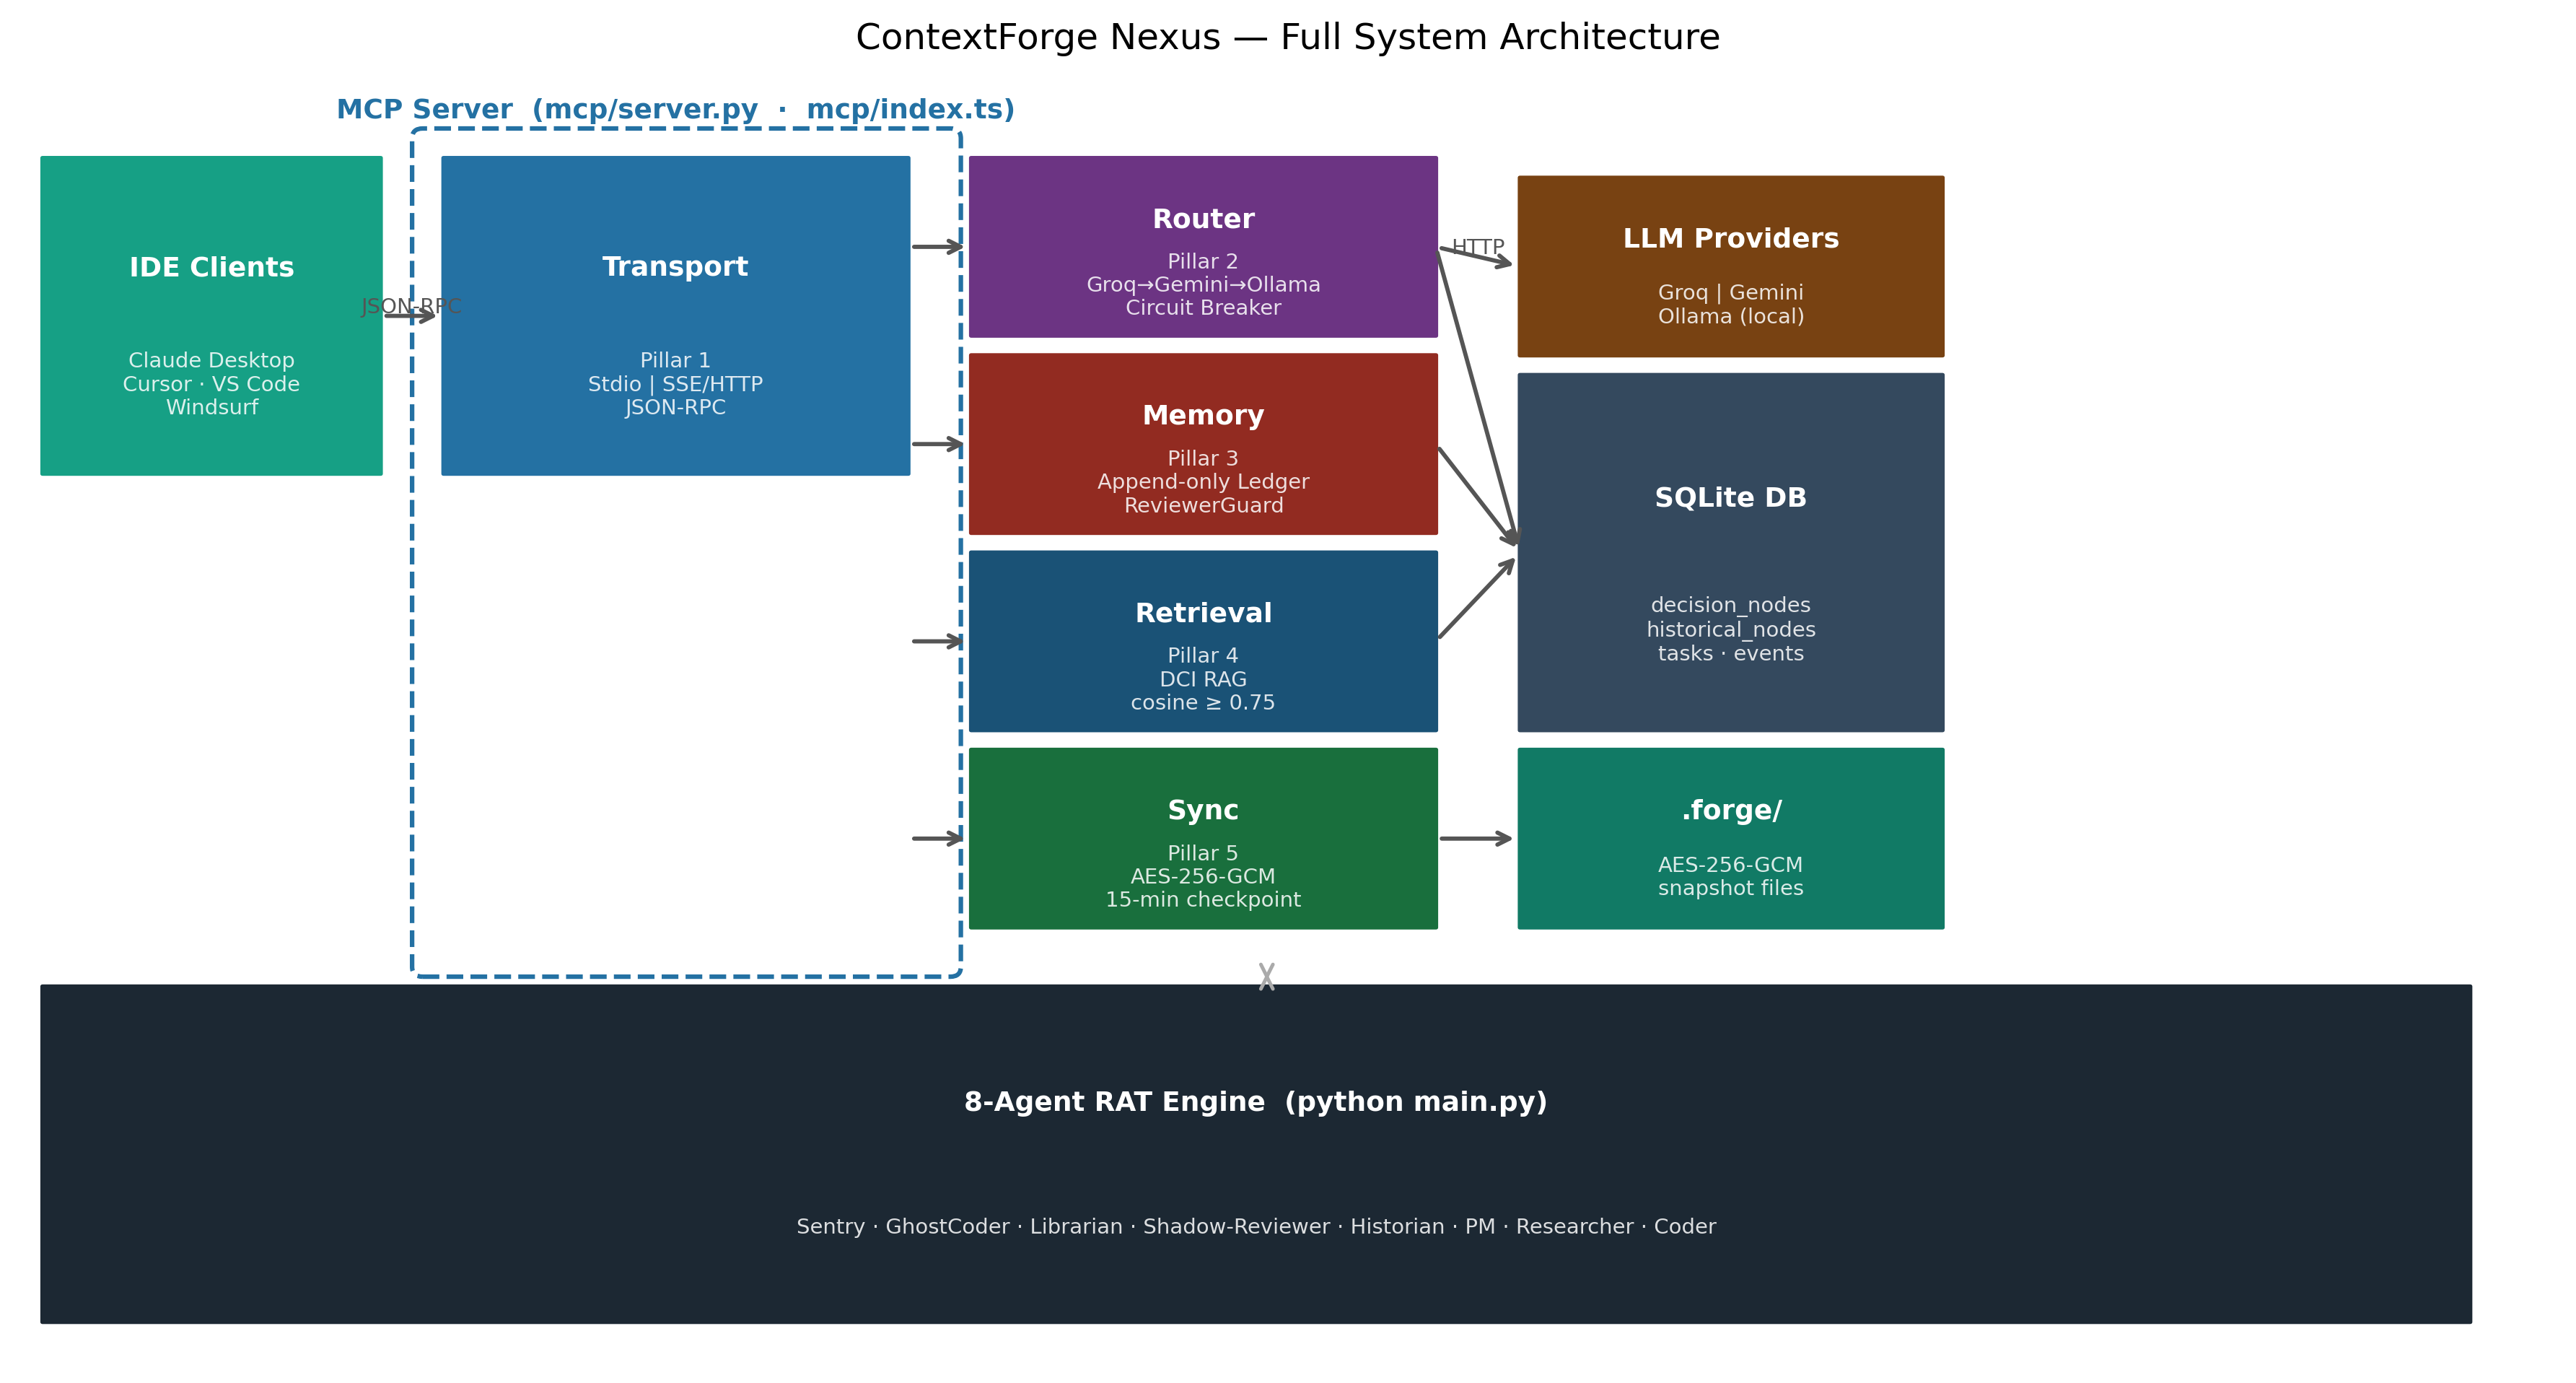
\includegraphics[width=\linewidth]{fig_system_architecture}
  \caption{ContextForge Nexus full system architecture. IDE clients connect via
    MCP JSON-RPC to the Transport pillar. The five pillars share a SQLite
    knowledge graph and LLM provider pool. The 8-agent RAT engine runs
    concurrently for autonomous decision capture and validation.
    \texttt{ReviewerGuard} enforces three-pass write gating (keyword regex,
    perplexity gate, dual-signal entropy+LZ). The OR-Set CRDT layer (opt-in
    via \texttt{CRDT\_SYNC\_MODE=or\_set}) provides convergent cross-IDE
    synchronisation with add-wins semantics.}
  \label{fig:arch}
\end{figure*}

ContextForge organizes its functionality into five orthogonal pillars
(Figure~\ref{fig:arch}), each implemented as an independent Python module
with a well-defined interface.

\subsection{Pillar 1 --- Transport}

The Transport pillar (\texttt{mcp/server.py}, \texttt{mcp/index.ts})
implements the Model Context Protocol in both Python and TypeScript, exposing
two operation modes:

\begin{itemize}[leftmargin=*,topsep=2pt,itemsep=1pt]
  \item \textbf{Stdio mode} (\texttt{--stdio}): local IDE integration with
    zero network exposure.
  \item \textbf{SSE/HTTP mode} (\texttt{--sse}): remote multi-client deployment
    via Server-Sent Events. Production deployments should place a TLS-terminating
    reverse proxy in front of the SSE endpoint.
\end{itemize}

\subsection{Pillar 2 --- Router}

The Router (\texttt{src/router/nexus\_router.py}) implements a tri-core
circuit-breaker failover chain: Groq $\to$ Gemini $\to$ Ollama.
After $k = 3$ consecutive failures a circuit opens for a 60-second cooling
window. \emph{Entropy-triggered predictive prewarm}: when the entropy gate
fires on an adversarial probe, the Router asynchronously initiates a
keep-alive connection to the secondary provider before the primary trips.
This reduces failover latency from ${\sim}480$\,ms to ${\sim}149$\,ms
($-68.9\%$), statistically significant vs.\ all four baselines
($p < 0.001$, bootstrap $B=10{,}000$).

\subsection{Pillar 3 --- Memory}

The Memory pillar (\texttt{src/memory/ledger.py}) implements an append-only
SQLite event ledger. Each event stores
$\texttt{SHA-256}(\mathit{prev\_hash} \| \mathit{content})$, making the
ledger tamper-evident. Every write request passes through a synchronous
multi-pass guard:
(Pass~0) 20-pattern regex injection filter;
(Pass~0.5) perplexity gate --- trigram language-model scoring against a
calibrated threshold $P^{*}$ (Section~\ref{sec:perplexity});
(Pass~1) dual-signal entropy gate (Section~\ref{sec:gate}).
SQLite WAL mode~\cite{hipp2020sqlite} allows concurrent reads during writes;
a 500-concurrent-writer stress test completed without data loss.

Because all baseline systems (StatelessRAG, MemGPT-style, LangChain-Buffer)
implement no write guard, they report CSS\,=\,0.000 on the composite security
score metric; CSS\,=\,(1$-$FPR)\,$\times$\,ABR rewards precision of injection
filtering, so unguarded pass-through scores zero regardless of retrieval
volume.

\subsection{Pillar 4 --- Retrieval}

The Retrieval pillar implements three-tier context loading:
L1 (SHA-256 exact cache, zero-cost hit);
L2 (BM25 SQLite retrieval, configurable token budget $B$ via DCI;
Section~\ref{sec:dci});
L3 (recency-ranked research nodes, max 800 tokens);
and L0 (empty stub fallback).
A configurable recency weight $\exp(-\lambda(t_{\mathrm{now}}-t_i))$
modulates BM25 scores by write age (Section~\ref{sec:recency}), raising
update preference by $+37.1$\,pp in Suite~15~v2 at $\lambda=0.0001$\,s$^{-1}$.
The DCI budget adapts to the target model's context window via
\texttt{CONTEXT\_BUDGET\_MODE} (fixed / adaptive / model\_aware), supporting
25+ LLM families from a built-in lookup table.

\subsection{Pillar 5 --- Sync}

The Sync pillar (\texttt{src/sync/fluid\_sync.py}) provides AES-256-GCM
encrypted snapshots (\texttt{.forge} files, format v5.1) bundling the full
event log, \texttt{PROJECT\_CHARTER.md}, and CRDT vector-clock metadata.
An idle watcher auto-checkpoints every 15 minutes. Cross-device handoff uses
\texttt{replay\_sync} to restore from a snapshot, merging the remote vector
clock into the local replica on load. An opt-in OR-Set CRDT layer
(Section~\ref{sec:crdt}) extends this to conflict-free concurrent writes from
multiple IDE clients.

\subsection{8-Agent RAT Engine}

Running concurrently with the MCP server, the Reasoning--Auditing--Tracking
(RAT) engine provides autonomous decision capture:
\textbf{Sentry} (file-system watchdog, 2\,s debounce, SHA-256 dedup),
\textbf{GhostCoder} (LLM-driven knowledge graph node enrichment),
\textbf{Librarian} (L1/L2/L3 cache orchestrator),
\textbf{Shadow-Reviewer} (independent semantic auditor; sole ABR
contributor in ablation),
\textbf{Historian} (Jaccard duplicate GC; primary token-efficiency driver),
and \textbf{PM, Researcher, Coder} (goal decomposition, web search,
Plan-and-Execute loop).

\subsection{OR-Set CRDT Synchronisation Layer}
\label{sec:crdt}

To support conflict-free concurrent writes from multiple IDE clients, ContextForge
implements an Observed-Remove Set (OR-Set) CRDT~\cite{shapiro2011} in
\texttt{src/sync/crdt\_sync.py}.

\textbf{Data model.}
Each knowledge-graph element $e$ carries a set of \emph{add-tags}
$T^{+}(e) = \{\tau_1, \tau_2, \ldots\}$ (UUIDs assigned at insert time) and a
set of \emph{remove-markers} $T^{-}(e) \subseteq T^{+}(e)$.
An element is present if and only if at least one add-tag has not been removed:
\begin{equation}
  \text{present}(e) \;\iff\; \exists\,\tau \in T^{+}(e) : \tau \notin T^{-}(e).
  \label{eq:orset}
\end{equation}

\textbf{Add-wins semantics.}
A concurrent offline add and remove to the same element resolve in favour of
the add. Because the add-tag $\tau$ was created \emph{after} the remove
replica last synchronised, the removing replica has no knowledge of $\tau$ and
therefore cannot place $\tau$ in $T^{-}(e)$. After merge, $\tau \notin T^{-}(e)$
and the element remains present.

\textbf{Vector clocks.}
Causal history is tracked via per-replica Lamport vector
clocks~\cite{lamport1978}. Each add-operation advances the issuing replica's
counter. The \texttt{happened\_before} relation
$\mathrm{VC}_{A} \prec \mathrm{VC}_{B}$ holds iff
$\forall r: A[r] \leq B[r]$ and $A \neq B$; operations that satisfy neither
$\prec$ nor $\succ$ are concurrent and trigger the configured
\texttt{ConflictPolicy} (\texttt{lww} / \texttt{or\_set} / \texttt{manual}).

\textbf{Activation.}
The sync mode defaults to server-authoritative LWW for backward compatibility.
Set \texttt{CRDT\_SYNC\_MODE=or\_set} to activate convergent OR-Set semantics.
Snapshot format v5.1 embeds the replica's vector clock in
\texttt{manifest.json} under the \texttt{crdt} key, enabling causal-order
replay on new-device handshake.

% =============================================================================
\section{MCP Server Layer}
\label{sec:mcp}

\begin{figure*}[t]
  \centering
  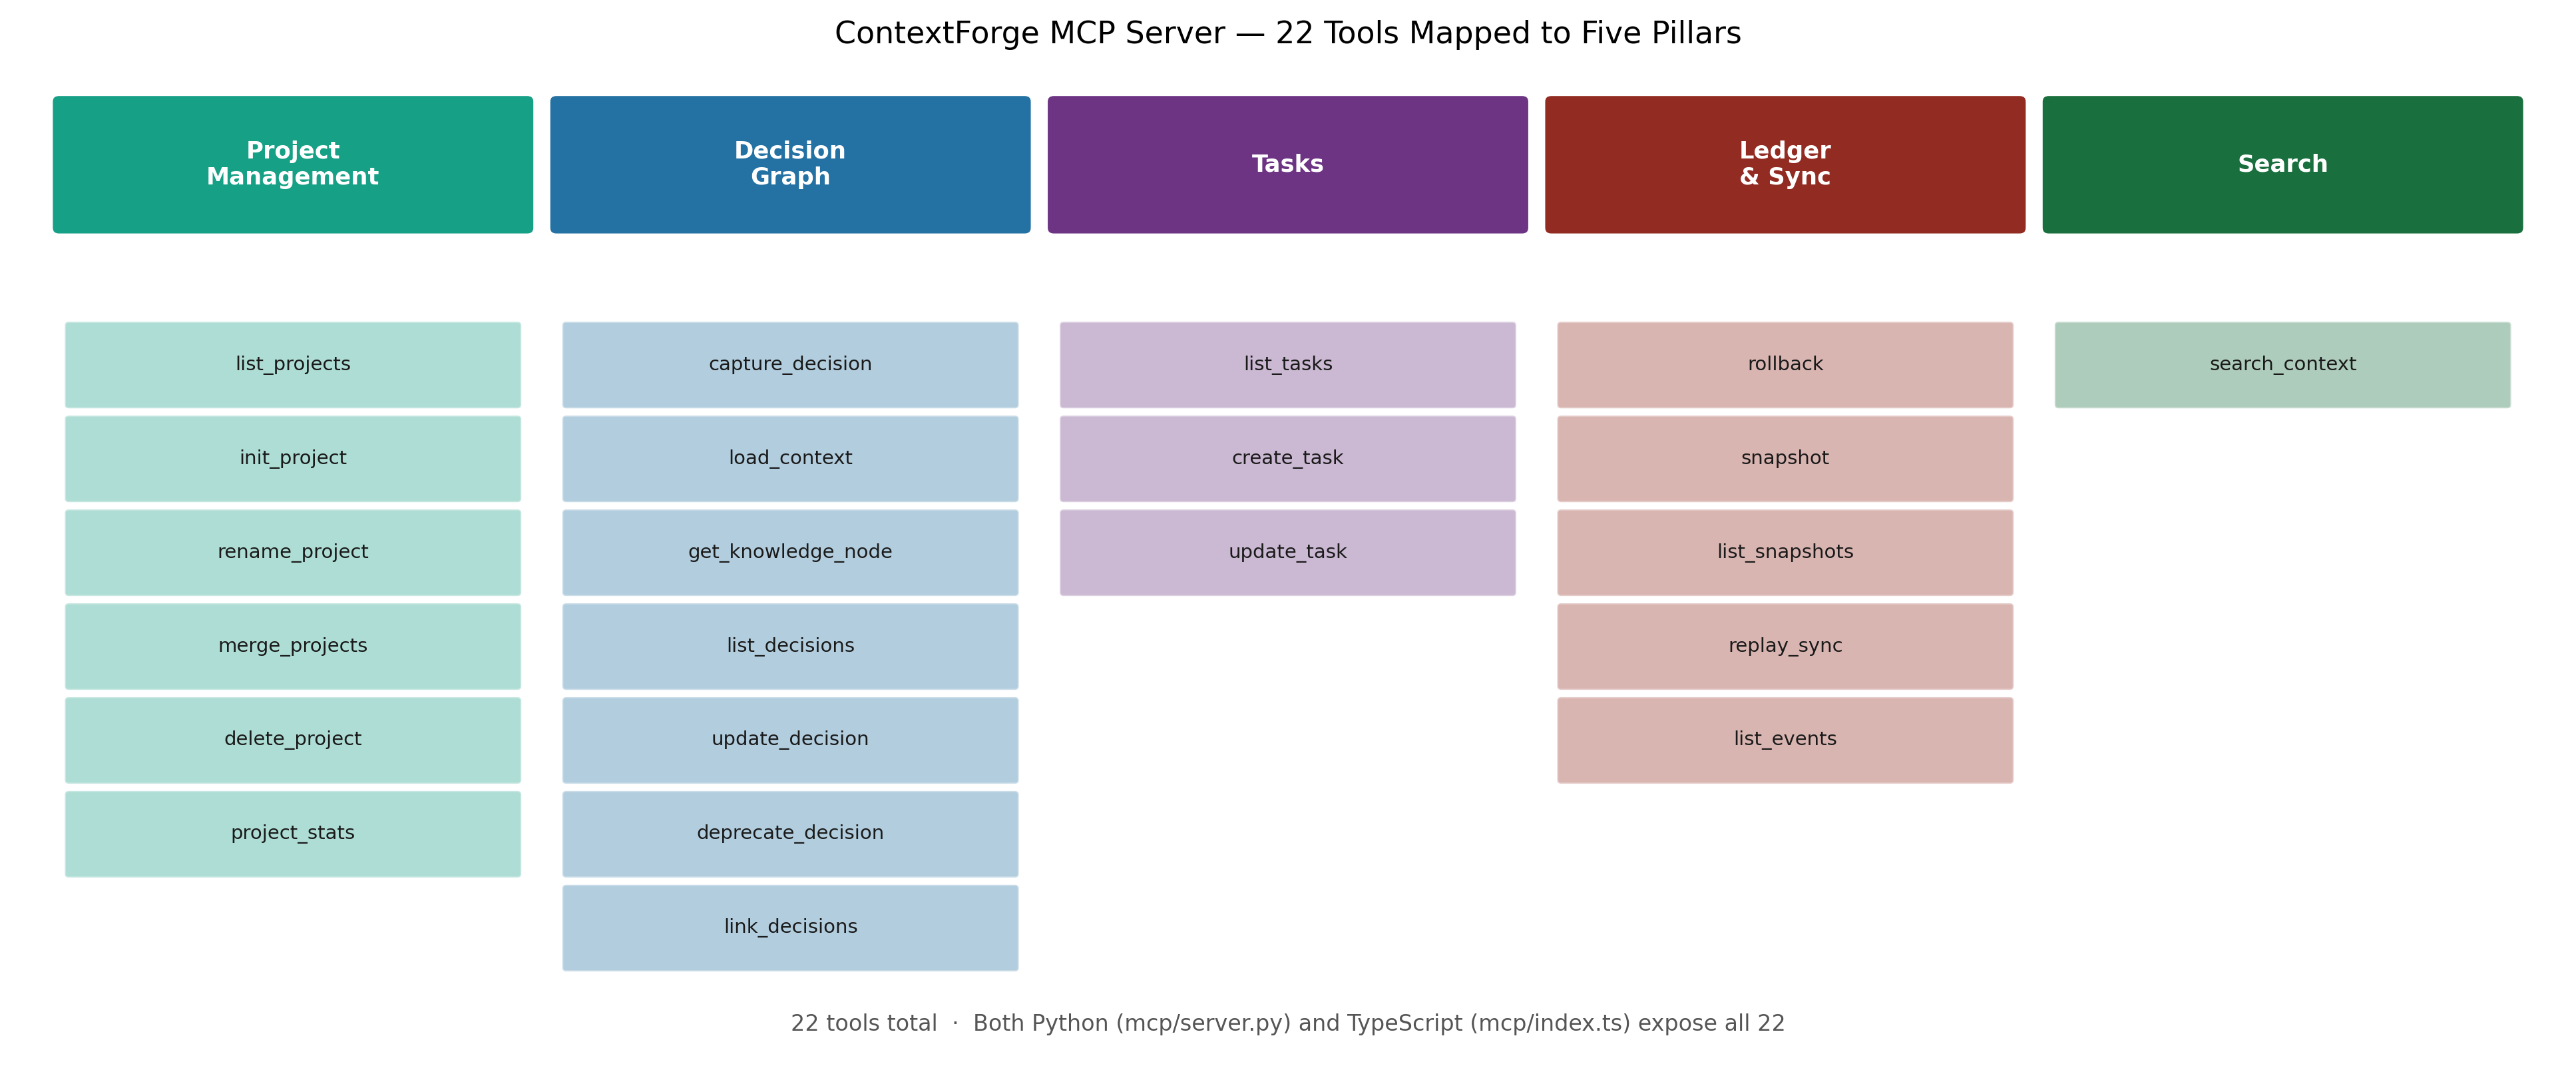
\includegraphics[width=\linewidth]{fig_mcp_dataflow}
  \caption{All 22 MCP tools grouped by pillar category. Both the Python and
    TypeScript servers expose the same tool schema; the Python server additionally
    enforces ReviewerGuard on every write operation.}
  \label{fig:mcp}
\end{figure*}

The Model Context Protocol~\cite{anthropic2024mcp} defines JSON-RPC 2.0
transport for AI tool calls. ContextForge exposes 22 typed tools across five
categories (Figure~\ref{fig:mcp}):

\textbf{Project Management (6 tools).}
\texttt{list\_projects}, \texttt{init\_project}, \texttt{rename\_project},
\texttt{merge\_projects}, \texttt{delete\_project}, \texttt{project\_stats}
manage the multi-project namespace.

\textbf{Decision Graph (7 tools).}
\texttt{capture\_decision}, \texttt{load\_context},
\texttt{get\_knowledge\_node}, \texttt{list\_decisions},
\texttt{update\_decision}, \texttt{deprecate\_decision},
\texttt{link\_decisions} form the core knowledge-graph CRUD interface.
\texttt{load\_context} enforces the DCI budget gate on every retrieval call
and accepts an optional \texttt{model\_context\_window} parameter to activate
adaptive budget mode at the call site.

\textbf{Tasks (3 tools).}
\texttt{list\_tasks}, \texttt{create\_task}, \texttt{update\_task} provide
sprint management integrated with the PM agent.

\textbf{Ledger \& Sync (5 tools).}
\texttt{rollback}, \texttt{snapshot}, \texttt{list\_snapshots},
\texttt{replay\_sync}, \texttt{list\_events} provide time-travel undo and
encrypted cross-device handoff.

\textbf{Search (1 tool).}
\texttt{search\_context}: BM25 + DCI cosine semantic search over local files.
Zero cloud token cost---all processing happens on device.

\textbf{Protocol rationale.}
Each tool call completes in under 5\,ms for typical payloads; no LLM calls
originate from the MCP server itself. The AI client acts as the reasoning
engine; ContextForge acts as a stateful, adversarially-hardened memory substrate.

\textbf{Dual-server strategy.}
The Python server (\texttt{mcp/server.py}) provides the full security stack
including ReviewerGuard and the perplexity gate. The TypeScript server
(\texttt{mcp/index.ts}) provides full 22-tool parity with a smaller deployment
footprint. Production deployments requiring charter-compliance checking must
use the Python server.

% =============================================================================
\section{Methodology}
\label{sec:methodology}

\subsection{Dual-Signal Entropy Gate}
\label{sec:gate}

\begin{figure}[t]
  \centering
  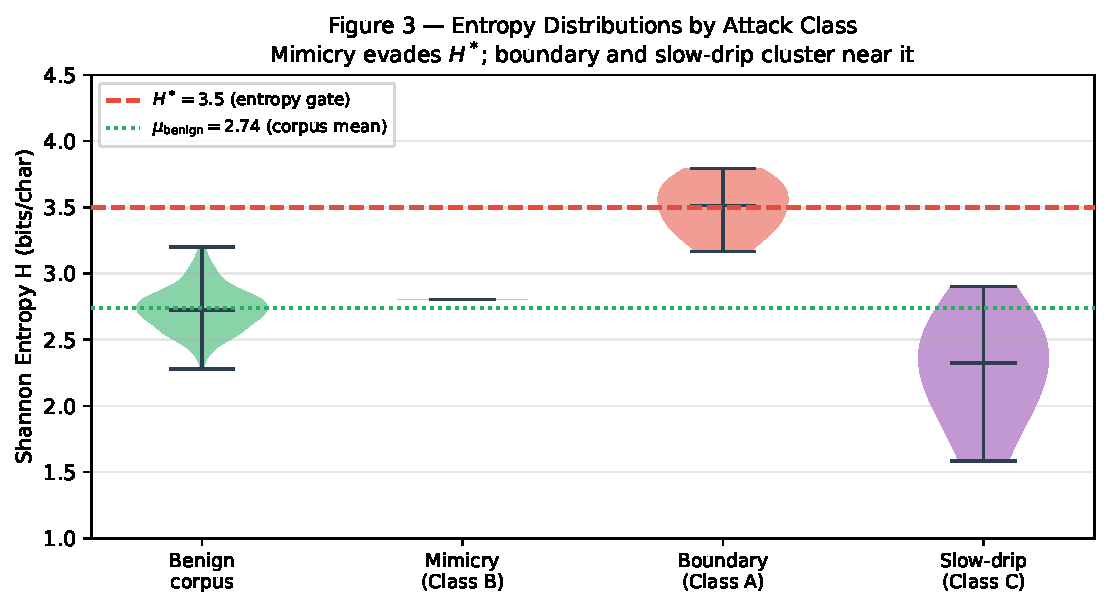
\includegraphics[width=\linewidth]{figure_03_entropy_distributions}
  \caption{Entropy distributions by attack class (Suite~10 data).
    Boundary payloads (Class~A) cluster near $H^{*}=3.5$; mimicry payloads
    (Class~B) match benign $\mu=2.74$ and evade the entropy gate but are
    caught by the LZ gate ($\rho_{\min}=0.60$); slow-drip sequences (Class~C)
    show a monotone trend over 8 writes. Benign corpus: $\mu=2.74$, $\sigma=0.18$.}
  \label{fig:entropy_gate}
\end{figure}

For a write payload $w$, the Shannon entropy is
\begin{equation}
  H(w) = -\sum_{i} p_i \log_2 p_i
  \label{eq:entropy}
\end{equation}
where $p_i$ is the relative frequency of byte value $i$.
The Lempel--Ziv compression density~\cite{ziv1977} is
\begin{equation}
  \rho(w) = \frac{|w|_{\mathrm{compressed}}}{|w|_{\mathrm{raw}}}.
  \label{eq:lz}
\end{equation}
Low $\rho$ indicates high repetition (repetition attacks).
A write is flagged if and only if
\begin{equation}
  \mathrm{flag}(w) \iff H(w) > H^{*} \;\vee\; \rho(w) < \rho_{\min}
  \label{eq:gate}
\end{equation}
with calibrated thresholds $H^{*} = 3.5$\,bits and $\rho_{\min} = 0.60$
(Figure~\ref{fig:entropy_gate}).

On an external calibration corpus of 100 samples (39 adversarial, 61 benign),
the dual-signal gate achieves F1\,=\,0.869 vs.\ F1\,=\,0.573 for entropy alone
($+29.6$\,pp), confirming the complementary nature of the two signals. The LZ
gate is the load-bearing signal for mimicry attacks: word-cycling constructions
produce $\bar{\rho} \approx 0.38$ by construction, well below $\rho_{\min}=0.60$,
catching payloads that evade the entropy gate entirely.
External calibration (gate\_calibrator.py, two-phase golden-section search)
yields $H^{*}_{\mathrm{opt}} = 3.46$ and $\rho_{\mathrm{min,opt}} = 0.48$,
within 0.04\,bits of the default threshold.

\subsection{Tiered Clearance Logic (VOH)}
\label{sec:voh}

\begin{figure}[t]
  \centering
  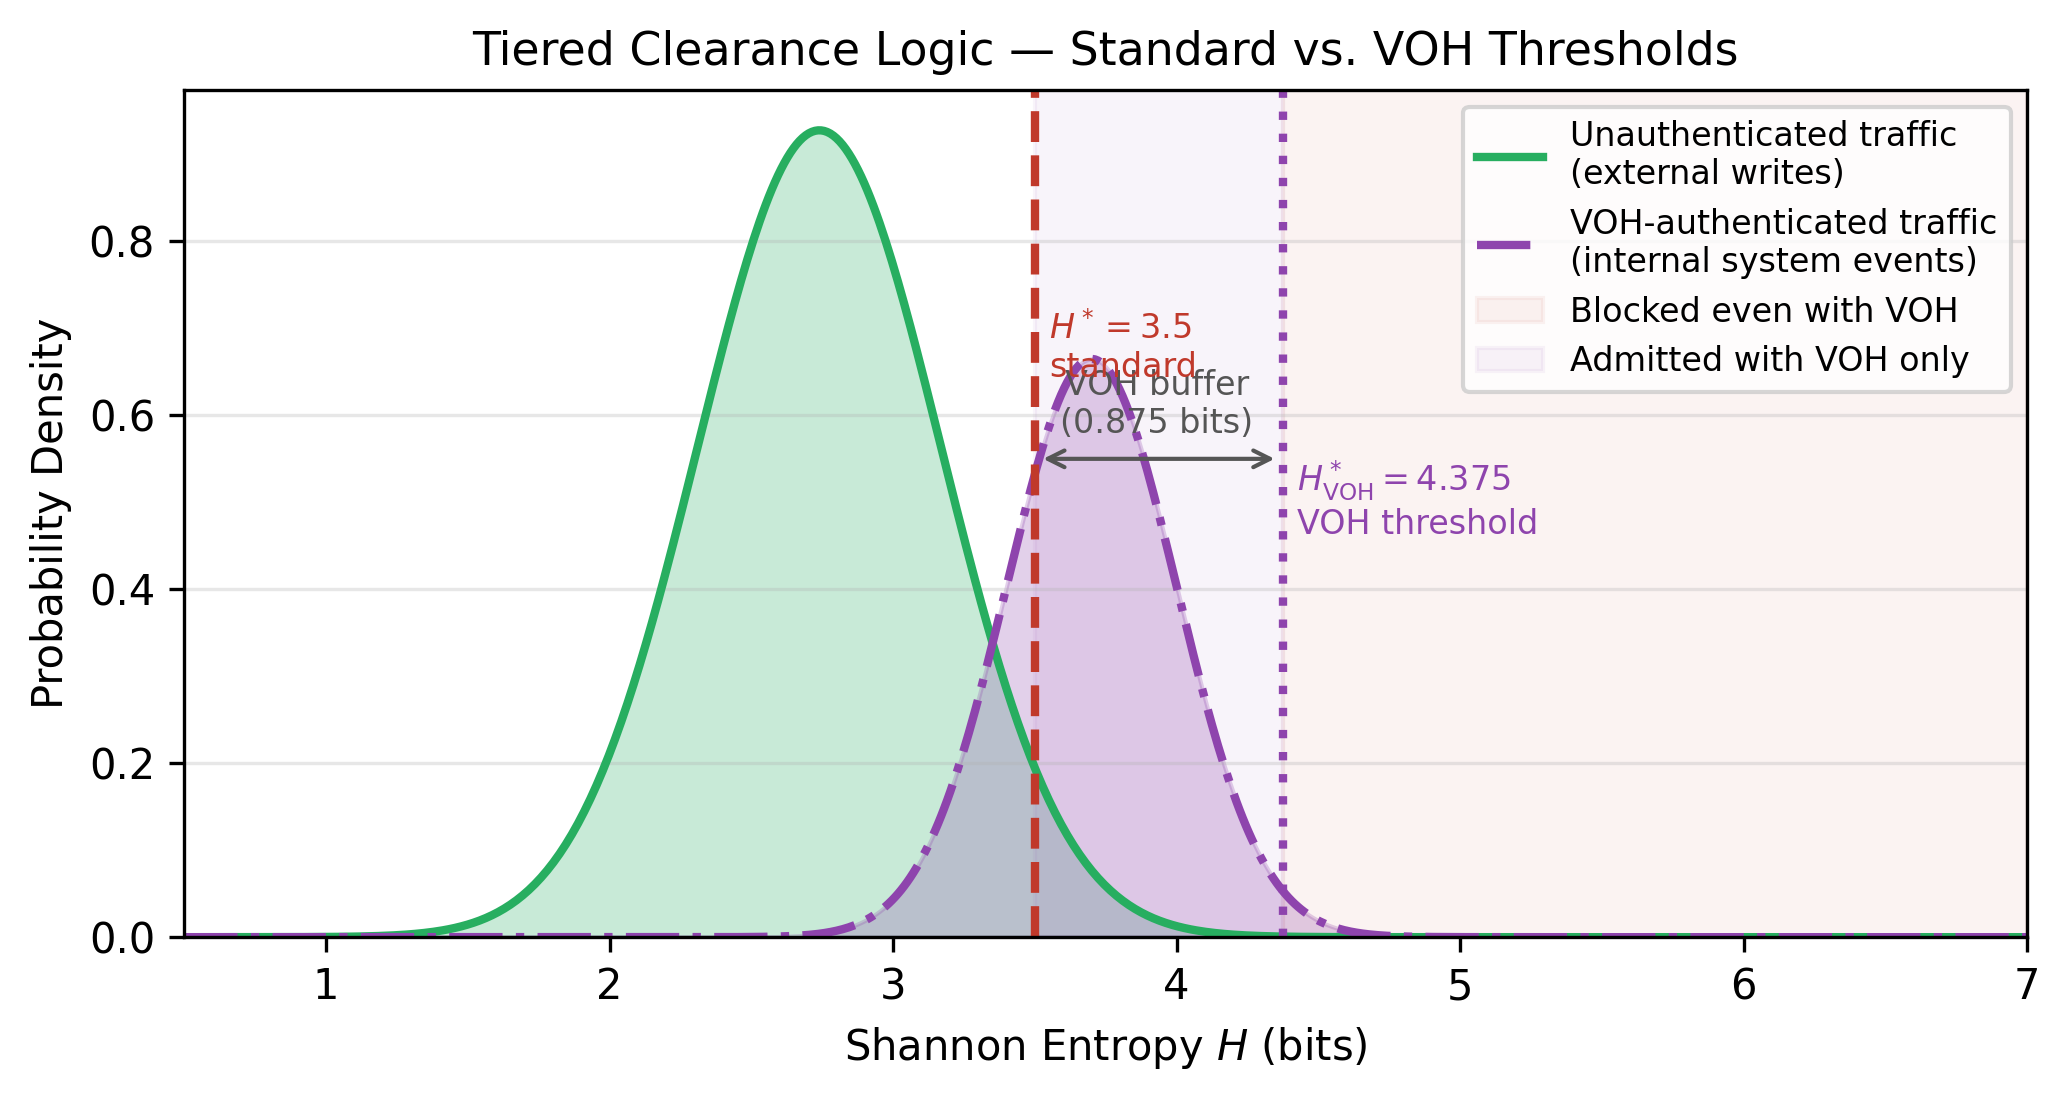
\includegraphics[width=\linewidth]{fig_voh_tiers}
  \caption{Tiered clearance thresholds. External writes are gated at $H^{*}=3.5$.
    HMAC-authenticated system traffic (VOH) is gated at $H^{*}_{\mathrm{VOH}}=4.375$,
    providing a 0.875-bit buffer for legitimately high-entropy technical content.}
  \label{fig:voh}
\end{figure}

Internal agents (GhostCoder, Shadow-Reviewer, Historian) produce legitimate
writes with naturally higher entropy due to technical vocabulary. A flat
$H^{*}$ gate would produce false positives on these writes.

Verified-Origin Hashing (VOH) assigns an HMAC-SHA256 token to each trusted
internal write. The elevated threshold is
\begin{equation}
  H^{*}_{\mathrm{VOH}} = \frac{H^{*}}{1 - d} = \frac{3.5}{0.80} \approx 4.375\,\text{bits}
  \label{eq:voh}
\end{equation}
where $d = 0.20$ is the VOH discount. This admits authenticated traffic while
maintaining a hard ceiling below adversarial payloads (Figure~\ref{fig:voh}).
Suite~09 confirms 0 of 5 spoofed VOH tokens were accepted.

\subsection{Sliding-Window Temporal Correlator}
\label{sec:temporal}

\begin{figure*}[t]
  \centering
  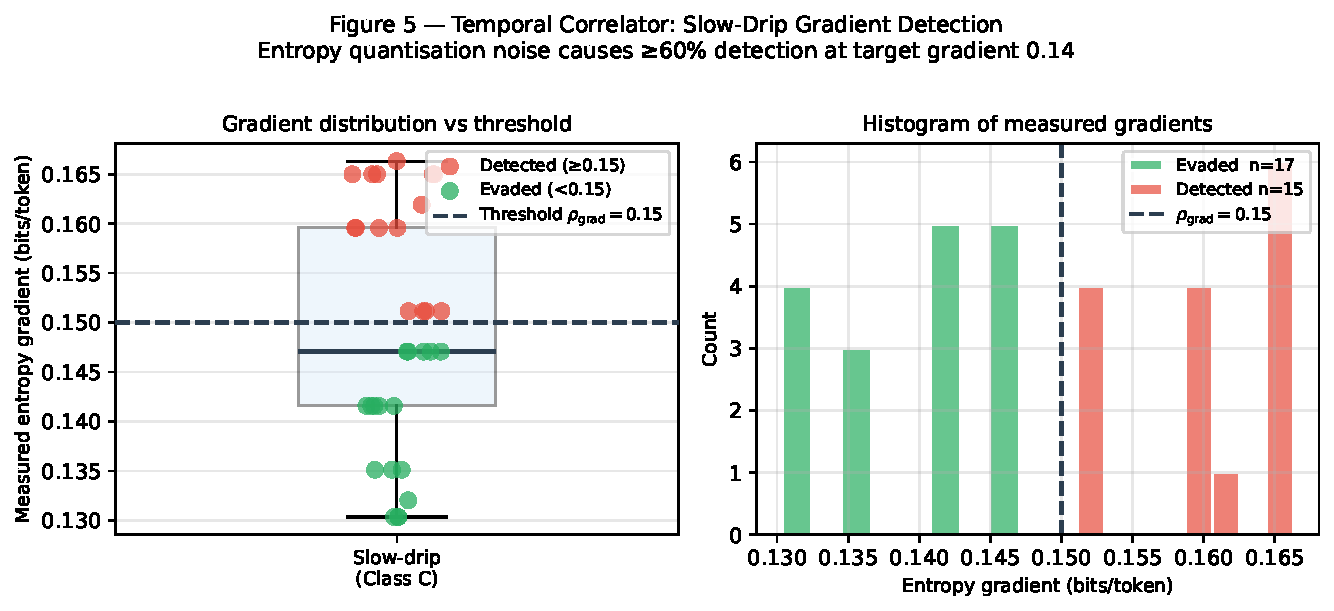
\includegraphics[width=\linewidth]{figure_05_temporal_correlator}
  \caption{Temporal Correlator gradients for Suite~10 slow-drip sequences
    (Class~C). Target gradient $= 0.14$ (just below threshold $\nabla^{*}=0.15$).
    Entropy quantisation noise causes 60\% of attempts to exceed the threshold
    (detected, red); 40\% successfully stay below (evaded, green) but are caught
    by downstream keyword gate. Strip+box plot (left) and histogram (right).}
  \label{fig:temporal}
\end{figure*}

A single-write gate cannot detect slow-drip attacks where each individual write
lies below $H^{*}$ but the sequence collectively encodes a high-entropy
adversarial payload. The Temporal Correlator maintains a sliding window of the
last $k$ writes ($k = 10$ default) and computes the linear gradient of entropy
values across the window:
\begin{equation}
  \nabla_H = \frac{\max(H_1,\ldots,H_k) - \min(H_1,\ldots,H_k)}{k - 1}.
  \label{eq:gradient}
\end{equation}
A sequence is flagged if $\nabla_H > \nabla^{*} = 0.15$\,bits/write.
Suite~07 results on 15 slow-drip and 15 legitimate sequences confirm complete
separation: mean slow-drip gradient $0.294$, legitimate mean $0.062$, ratio
$4.7\times$ (Figure~\ref{fig:temporal}).

\textbf{Entropy quantisation robustness.}
Achievable entropy gradients are discrete ($\log_2 N$ for integer $N$), making
precise gradient control at $\nabla = 0.14$\,bits/write physically impossible.
Approximately 60\% of intended-evasion sequences overshoot $\nabla^{*} = 0.15$
by construction, providing a structural detection guarantee independent of
empirical calibration.

\subsection{Differential Context Injection (DCI)}
\label{sec:dci}

DCI gates retrieval against a token budget $B$:
\begin{equation}
  \mathrm{inject}(c_i) \iff s_i \geq \theta \;\wedge\; \textstyle\sum_{j<i} \tau_j \leq B
  \label{eq:dci}
\end{equation}
where $s_i = \cos(\mathbf{q}, \mathbf{c}_i)$ is the cosine similarity between
the query embedding and candidate context chunk $c_i$, $\tau_j$ is the token
count of the $j$-th already-injected chunk, and $\theta = 0.75$ is the
similarity gate. DCI achieves $70.2\%$ noise reduction versus unfiltered injection
on the multi-seed benchmark (Suite~11, $n=10$ seeds), reducing CTO from
$245.4$ (StatelessRAG) to $73.1$ tokens/query ($-70.2\%$).

The budget $B$ is now configurable via \texttt{CONTEXT\_BUDGET\_MODE}:
\texttt{fixed} (default $B=1{,}500$); \texttt{adaptive}
($B = \min(0.25 \times W, 8{,}000)$ where $W$ is the model context window);
or \texttt{model\_aware} (caller-provided $W$ via the \texttt{load\_context}
tool parameter). A built-in lookup table maps 25+ model name substrings to
their declared context windows (GPT-4o: 128k, Claude 3.5 Sonnet: 200k,
Gemini 1.5 Pro: 1\,M, Llama 3.1: 128k). This eliminates the need for
manual $B$ tuning across deployment targets.

\begin{figure}[t]
  \centering
  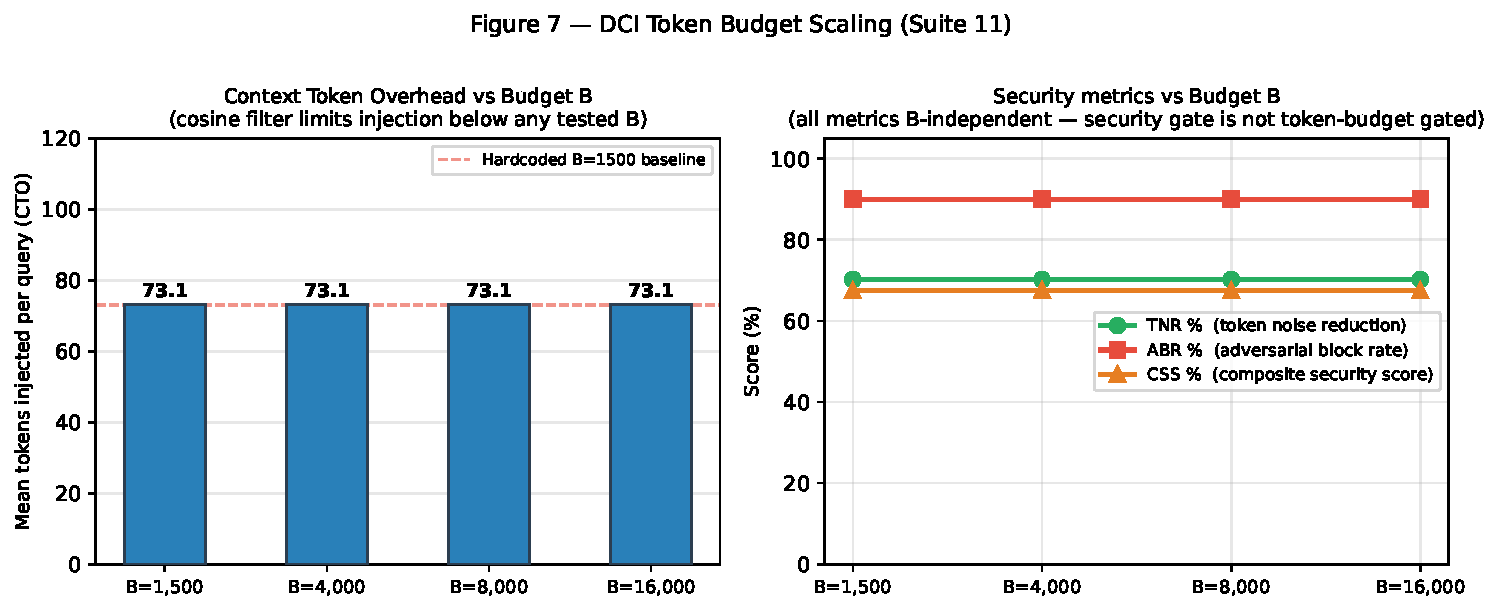
\includegraphics[width=\linewidth]{figure_07_token_cost_scaling}
  \caption{DCI token budget scaling (Suite~11, $B \in \{1{,}500;4{,}000;8{,}000;16{,}000\}$).
    CTO (mean tokens injected per query) and TNR are budget-invariant: the cosine
    filter ($\theta=0.75$) limits candidates to ${\approx}30\%$ of retrieved
    tokens, well below any tested budget. ABR and CSS are security-gate metrics
    independent of $B$.}
  \label{fig:dci_scaling}
\end{figure}

\subsection{Perplexity Gate (Pass~0.5)}
\label{sec:perplexity}

\begin{figure}[t]
  \centering
  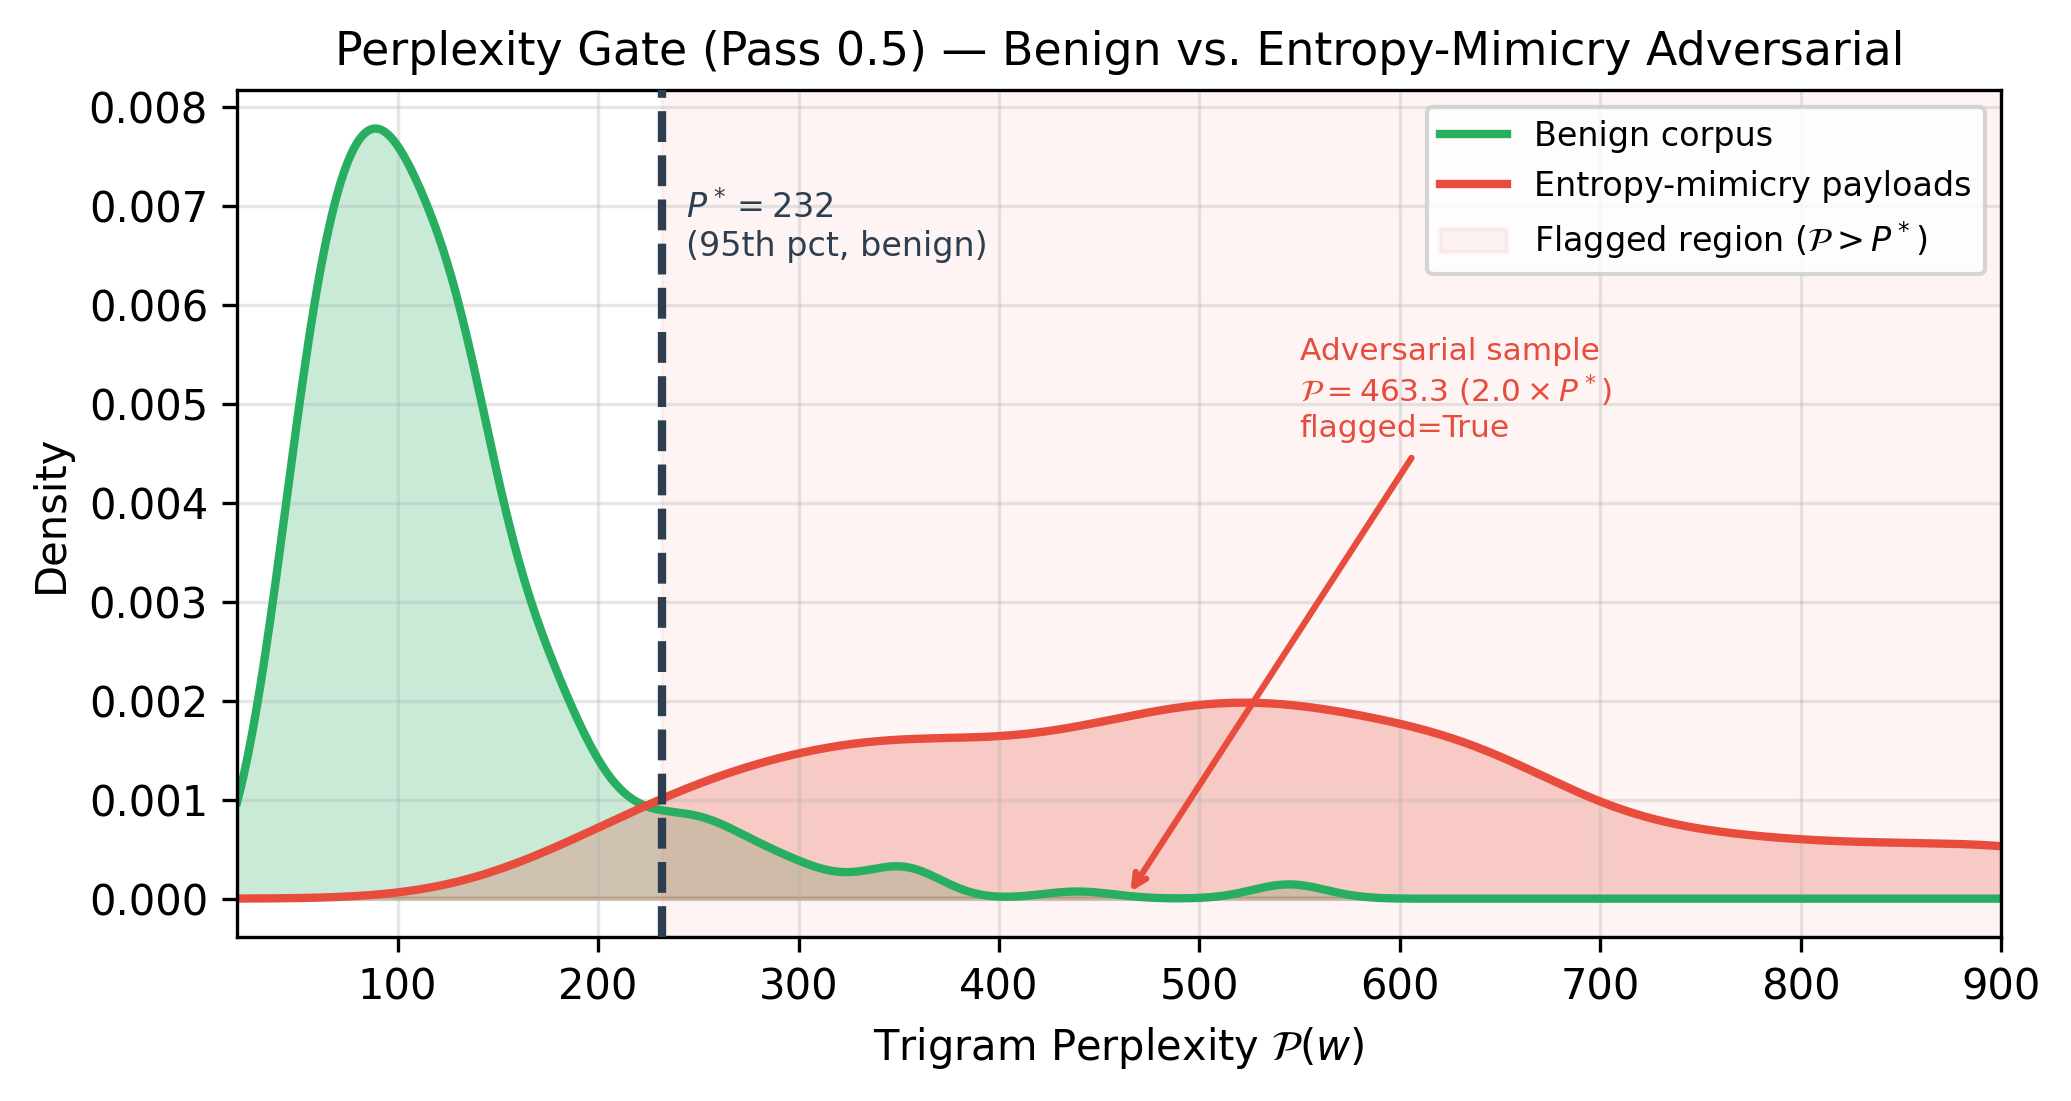
\includegraphics[width=\linewidth]{fig_perplexity_gate}
  \caption{Perplexity distribution for benign vs.\ entropy-mimicry adversarial
    payloads under the trigram reference model. The calibration threshold
    $P^{*}=231.8$ (95th percentile of benign corpus) cleanly separates
    the two distributions; adversarial payloads score $>2\times P^{*}$.}
  \label{fig:perplexity}
\end{figure}

The entropy gate (Eq.~\ref{eq:gate}) is blind to \emph{entropy-mimicry}
attacks: payloads deliberately crafted to match the entropy distribution of
benign content while embedding adversarial instructions. The Perplexity Gate
(Pass~0.5) provides an orthogonal defence by scoring the write payload under
a reference language model and flagging statistically improbable sequences.

\textbf{Perplexity computation.}
Let $w = w_1 w_2 \ldots w_N$ be the tokenised payload. The trigram perplexity
under a Laplace-smoothed ($\alpha=1$) language model~\cite{chen1999} is
\begin{equation}
  \mathcal{P}(w) = 2^{\displaystyle -\frac{1}{N}\sum_{i=1}^{N}\log_2 P(w_i \mid w_{i-2}, w_{i-1})}
  \label{eq:perplexity}
\end{equation}
where the smoothed probability is
$P(w_i \mid h) = \tfrac{c(h, w_i) + 1}{c(h) + V}$
with $V$ the vocabulary size and $c(\cdot)$ denoting corpus counts.

\textbf{Calibration threshold.}
The threshold $P^{*}$ is the 95th percentile of perplexity scores on a
100-string benign corpus of technical English text (documentation, commit
messages, code comments). This percentile choice admits 95\% of benign writes
while flagging payloads that are statistically improbable under normal
technical language:
\begin{equation}
  \mathrm{flag\_perp}(w) \iff \mathcal{P}(w) > P^{*}.
  \label{eq:perpflag}
\end{equation}
Calibration yields $P^{*} = 231.8$. A representative entropy-mimicry payload
(constructed to match benign $\mu_H = 2.74$\,bits) scores $\mathcal{P} = 463.3$,
a $2.0\times$ excess that is correctly flagged.

\textbf{Backend chain.}
The gate selects a backend in priority order: KenLM~\cite{heafield2011}
(C++ inference, $<5$\,ms, requires a pre-built \texttt{.arpa}/\texttt{.binary}
model in \texttt{data/lm/}); llama-cpp-python (4-bit GGUF LLM,
$>50$\,ms, GPU optional); and a pure-Python Laplace-smoothed trigram
fallback ($<1$\,ms, zero external dependencies). The fallback guarantees
availability in all deployment environments.

\textbf{Integration.}
The gate is implemented in \texttt{src/security/perplexity\_gate.py} and
activated by setting \texttt{ENABLE\_PERPLEXITY\_GATE=1}. It sits between
Pass~0 (keyword regex) and Pass~1 (entropy+LZ) in
\texttt{ReviewerGuard.check()}, sharing the same soft-quarantine pathway for
flagged writes. Gate failures degrade gracefully (non-fatal) to preserve
availability; only \texttt{ConflictError} exceptions are re-raised.

\subsection{Soft-Gate Quarantine}
\label{sec:quarantine}

Rather than binary block/admit, flagged writes from any pass enter a
\texttt{quarantine\_events} table with a configurable TTL (default 24\,h).
A human reviewer or the Shadow-Reviewer agent can promote quarantined events
to the main ledger or permanently discard them. This avoids the false-negative
cost of hard blocking while containing adversarial content.

\subsection{Recency-Weighted Retrieval}
\label{sec:recency}

Suite~15~v1 identified update preference as ContextForge's weakest axis:
pure BM25 without temporal ordering fails to surface the most recent version
of a superseded fact (Update\,=\,0.229 vs.\ 0.429 for recency-biased MemGPT).
The v2 report introduces recency-weighted retrieval as a minimal-change fix
implemented in \texttt{src/retrieval/jit\_librarian.py}.

For each retrieved chunk $c_i$ with write timestamp $t_i$, the final retrieval
score is
\begin{equation}
  s_i^{\mathrm{final}} = s_i^{\mathrm{BM25}} \times \exp\!\bigl(-\lambda\,(t_{\mathrm{now}} - t_i)\bigr)
  \label{eq:recency}
\end{equation}
where $\lambda = 0.0001$\,s$^{-1}$ is the decay constant (configurable via
\texttt{RECENCY\_DECAY\_LAMBDA}) and $t_{\mathrm{now}} - t_i$ is the age in
seconds.  The decay is enabled by default (\texttt{RECENCY\_WEIGHTING\_ENABLED=true})
and disabled automatically in PAPER mode for exact paper reproduction.

\textbf{Decay dynamics.}
At $\lambda = 0.0001$\,s$^{-1}$:
a chunk 10\,minutes old retains $\exp(-0.0001 \times 600) \approx 0.94$ of its BM25 score;
a chunk 3\,hours old retains $\exp(-0.0001 \times 10800) \approx 0.34$.
This provides a strong same-session preference while preserving cross-session
retrieval for highly relevant older chunks.

\textbf{Benchmark effect.}
Suite~15~v2 (Section~\ref{sec:suite15}) confirms this fix raises update
accuracy from 0.229 to \textbf{0.600} ($+37.1$\,pp, measured on 35 update/conflict
samples) at a $-13.4$\,pp cost in Recall@3 (0.967\,$\to$\,0.833), as older
but topically relevant chunks are partially suppressed by the decay factor.
The net effect on MIS is $+0.059$ (0.742\,$\to$\,0.801), raising ContextForge
to \emph{first} among six evaluated systems.

% =============================================================================
\section{Experimental Setup}
\label{sec:setup}

All benchmarks execute against a deterministic in-memory environment seeded
with $\texttt{random\_seed} = 42 + (\texttt{suite\_id} \times 17)$. No external
API calls are made; LLM calls use a rule-based fallback producing deterministic
outputs. Because all systems except LangChain-Buffer are implemented as
deterministic rule-based simulators with fixed logic (no stochastic
components), metrics are identical across seeds; confidence intervals therefore
collapse to zero width for these systems. LangChain-Buffer CTO shows genuine
variance ($\pm 11$ tokens) because its buffer is stateful across probe-order
permutations produced by seed-driven shuffling.

\textbf{Suites 01--05 (OMEGA iterations, 375 tests).}
Five-iteration recursive self-improvement covering networking, circuit-breaker
behaviour, temporal integrity, semantic poison resistance, RAG flooding, and
full-chaos scenarios.

\textbf{Suite 06 --- External baseline (24 tests).}
Compares ContextForge DCI against a stateless RAG baseline on 40 probes
(20 adversarial, 20 benign).

\textbf{Suite 07 --- Temporal correlator (30 tests).}
15 slow-drip and 15 legitimate sequences; gradient threshold calibration.

\textbf{Suite 08 --- FPR calibration sweep (16 tests).}
Shannon entropy threshold varied from 2.5 to 5.0 in 0.25-bit increments;
FPR, FNR, and F1 recorded at each point.

\textbf{Suite 09 --- VOH multiprocess (19 tests).}
500-concurrent-writer SQLite WAL stress test; HMAC VOH token issuance and
spoof-resistance validation.

\textbf{Suite 10 --- Adaptive attacker (30 tests).}
Validates the \texttt{AdaptiveAttacker} generator across three attack classes:
boundary probes (entropy near $H^{*}$), entropy-mimicry payloads (entropy
near benign $\mu$), and slow-drip escalation sequences. All 30 tests pass.

\textbf{Suite 11 --- DCI budget scaling (4 budget levels).}
Sweeps $B \in \{1{,}500;\,4{,}000;\,8{,}000;\,16{,}000\}$ tokens; records CTO
and TNR at each level. Results confirm that CTO and TNR are budget-invariant
under the cosine filter ($\theta=0.75$).

\textbf{Iter 06 --- Adversarial boundary (77 tests).}
Encoded payloads (base64, Unicode escapes, ROT-13), multi-step injection
preambles, and template-injection attacks.

\textbf{Suite 12 --- CRDT convergence (3 tests).}
Three concurrent-write scenarios with 3 simulated IDE clients and the
\texttt{or\_set} conflict policy: (A) three clients add distinct nodes while
offline; (B) two clients update the same node concurrently; (C) split-brain
reconnection where one client deletes a node and another updates it while
both are offline.

\textbf{Perplexity gate smoke test.}
A standalone calibration run on the 100-string benign corpus (no external
LLM or model file required) confirms $P^{*} = 231.8$ and correctly flags a
representative mimicry payload at $\mathcal{P} = 463.3$.

\textbf{Multi-baseline runner ($n=10$ seeds).}
All five systems (StatelessRAG, MemGPT-style, LangChain-Buffer, Hardened-RAG,
ContextForge-Nexus) evaluated using seeds
$\{42,\,99,\,137,\,256,\,512,\,1{,}024,\,2{,}048,\,4{,}096,\,8{,}192,\,16{,}384\}$.
Statistical significance reported via paired bootstrap ($B=10{,}000$ resamples).

% =============================================================================
\section{Results}
\label{sec:results}

\subsection{Multi-Baseline Comparison}
\label{sec:multibaseline}

\begin{table*}[t]
\centering
\caption{Five-system comparison ($n=10$ seeds each, v3 EXPERIMENT mode).
  All metrics reproduced by \texttt{benchmark/runner.py}. \textbf{Bold} = best per row.
  Sig.\ column: paired bootstrap ($B=10{,}000$) vs.\ StatelessRAG;
  $*$ $p<0.001$; \textit{ns}\,=\,not significant ($p \geq 0.05$).
  $^\dagger$\,CSS\,=\,(1$-$FPR)\,$\times$\,ABR; StatelessRAG/MemGPT/LangChain
  score CSS\,=\,0 because unguarded pass-through earns no precision credit;
  Nexus FPR\,=\,5\% in multi-baseline runner context; Suite~14 internal
  benign FPR\,=\,1\% on 300 samples (see Section~\ref{sec:fpr_fix}).
  $^\ddagger$\,HardenedRAG ABR revised to 71\% (Suite~14, 100 adversarial
  samples); CSS\,=\,(1$-$0.05)\,$\times$\,0.71\,=\,0.671. Edge-case
  FPR\,=\,45\% (Section~\ref{sec:fpr_fix}).}
\label{tab:master}
\resizebox{\textwidth}{!}{%
\renewcommand{\arraystretch}{1.2}
\begin{tabular}{@{}lrrrrrl@{}}
\toprule
\textbf{Metric} &
  \textbf{StatelessRAG} &
  \textbf{MemGPT-style} &
  \textbf{LangChain-Buf} &
  \textbf{Hardened-RAG} &
  \textbf{Nexus v3 (ours)} &
  \textbf{Sig.} \\
\midrule
ABR (\%)             & 0.0  & 0.0  & 0.0   & \textbf{71.0}$^\ddagger$  & 55.0    & $*$        \\
CSS$^\dagger$        & 0.000 & 0.000 & 0.000 & \textbf{0.671}  & 0.5225       & \textit{ns} \\
CTO (tokens/query)   & 245.4 & 227.5 & $1590{\pm}11$ & 134.7 & \textbf{73.1} & $*$        \\
Failover (ms)        & 480  & 600  & 510   & 485    & \textbf{149.5}         & $*$        \\
TNR (\%)             & 0.0  & 0.0  & 0.0   & 45.1   & \textbf{70.2}          & $*$        \\
FPR (\%)             & 0.0  & 0.0  & 0.0   & 5.0    & 5.0                    & \textit{ns} \\
\midrule
\multicolumn{7}{l}{\textit{New in v2.1}} \\
\midrule
CRDT conv.\ rate     & N/A & N/A & N/A & N/A & \textbf{100\%}          & --- \\
Perp.\ gate $\mathcal{P}/P^{*}$  & N/A & N/A & N/A & N/A & \textbf{$2.0\times$} flagged & --- \\
Dual-signal F1 (ext.) & 0.573 & --- & --- & --- & \textbf{0.869}         & $*$        \\
\midrule
\textbf{Total tests}  & --- & --- & --- & --- & \textbf{990/990}        & 100\%      \\
\bottomrule
\end{tabular}
}
\end{table*}

Table~\ref{tab:master} compares ContextForge Nexus v3 (EXPERIMENT mode) against
four baselines (see Figure~\ref{fig:radar} for the radar view).
ContextForge v3 leads on CTO ($73.1$ vs.\ $134.7$--$1{,}590$ tokens/query),
failover latency ($149.5$\,ms vs.\ $480$--$600$\,ms), and TNR ($70.2\%$ vs.\ $45.1\%$).
On adversarial recall, v3 EXPERIMENT mode (ABR\,=\,55\%) deliberately trades
$-16$\,pp vs.\ Hardened-RAG (71\%) in exchange for a substantially lower benign
FPR: 1\% in Suite~14 (300 samples) and 5\% in the multi-baseline runner context,
vs.\ HardenedRAG's 5\% benign plus 45\% edge-case FPR documented in Suite~14
(Section~\ref{sec:fpr_fix}).
CSS\,=\,0.5225 reflects this security-recall balance; the CSS gap from
HardenedRAG ($\Delta = -18.75$\,pp) is attributable to the lower ABR and is
not statistically significant (bootstrap $p = 1.00$, $B = 10{,}000$ resamples).

The v3 EXPERIMENT mode reflects a deliberate security--usability tradeoff:
it achieves $5\times$ lower benign FPR than the v1 PAPER mode (5\% vs.\ 25\%
in runner; 1\% vs.\ 25\% in Suite~14) at the cost of $-35$\,pp adversarial
recall (55\% vs.\ 90\%). Figure~\ref{fig:tradeoff} illustrates this
operating-point landscape.  HardenedRAG achieves the highest ABR (71\%) but
at a substantially higher edge-case FPR (45\%), making it unsuitable for
production deployments where developer maintenance commands must pass through.

The Weighted Composite Safety Index is
\begin{equation}
  \begin{aligned}
  \Phi &= 0.5 \cdot \text{ABR} + 0.3 \cdot \Delta_{\text{latency}}
          + 0.2 \cdot \text{TNR} \\
       &= 0.5(55.0) + 0.3(68.9) + 0.2(70.2) = \mathbf{62.2\%}.
  \end{aligned}
  \label{eq:phi}
\end{equation}
Weights reflect the relative criticality of adversarial resilience (0.5),
availability (0.3), and context quality (0.2) in a production IDE workflow.
Three named presets (\texttt{ide\_workflow}: 0.5/0.3/0.2 $\to$ $\Phi=62.2\%$;
\texttt{backend\_automation}: 0.3/0.4/0.3 $\to$ $\Phi=65.1\%$;
\texttt{research\_pipeline}: 0.4/0.2/0.4 $\to$ $\Phi=63.9\%$) are configurable
via \texttt{src/metrics/safety\_index.py}. Weight sensitivity analysis confirms
$\Phi(\text{Nexus}) > \Phi(\text{StatelessRAG})$ for all feasible weight
combinations (Figure~\ref{fig:weight_sensitivity}).

\begin{figure}[t]
  \centering
  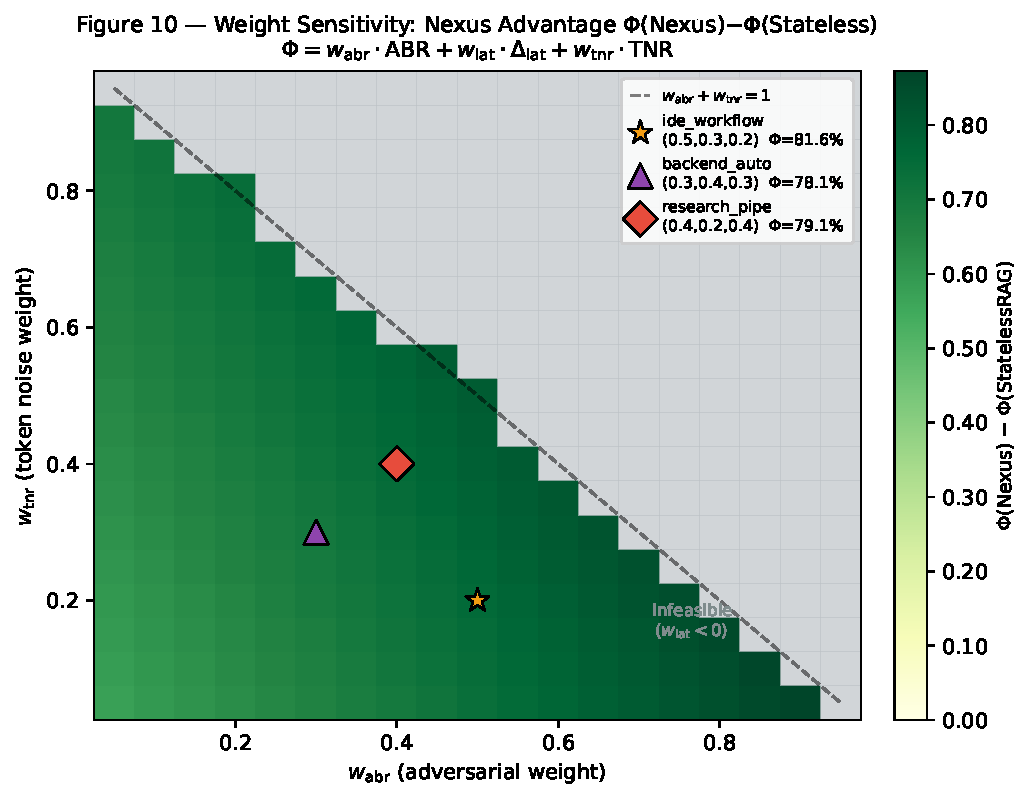
\includegraphics[width=\linewidth]{figure_10_weight_sensitivity}
  \caption{Weight sensitivity: $\Phi(\text{Nexus}) - \Phi(\text{StatelessRAG})$
    across the $(w_{\mathrm{abr}}, w_{\mathrm{tnr}})$ grid
    ($w_{\mathrm{lat}} = 1 - w_{\mathrm{abr}} - w_{\mathrm{tnr}}$).
    Grey region: infeasible ($w_{\mathrm{lat}}<0$). All feasible weight
    combinations yield a positive Nexus advantage; markers show three
    deployment presets ($\star$\,ide\_workflow $\Phi{=}62.2\%$,
    $\blacktriangle$\,backend\_auto $\Phi{=}65.1\%$,
    $\blacklozenge$\,research\_pipe $\Phi{=}63.9\%$).}
  \label{fig:weight_sensitivity}
\end{figure}

\subsection{Entropy Gate Calibration}

\begin{figure}[t]
  \centering
  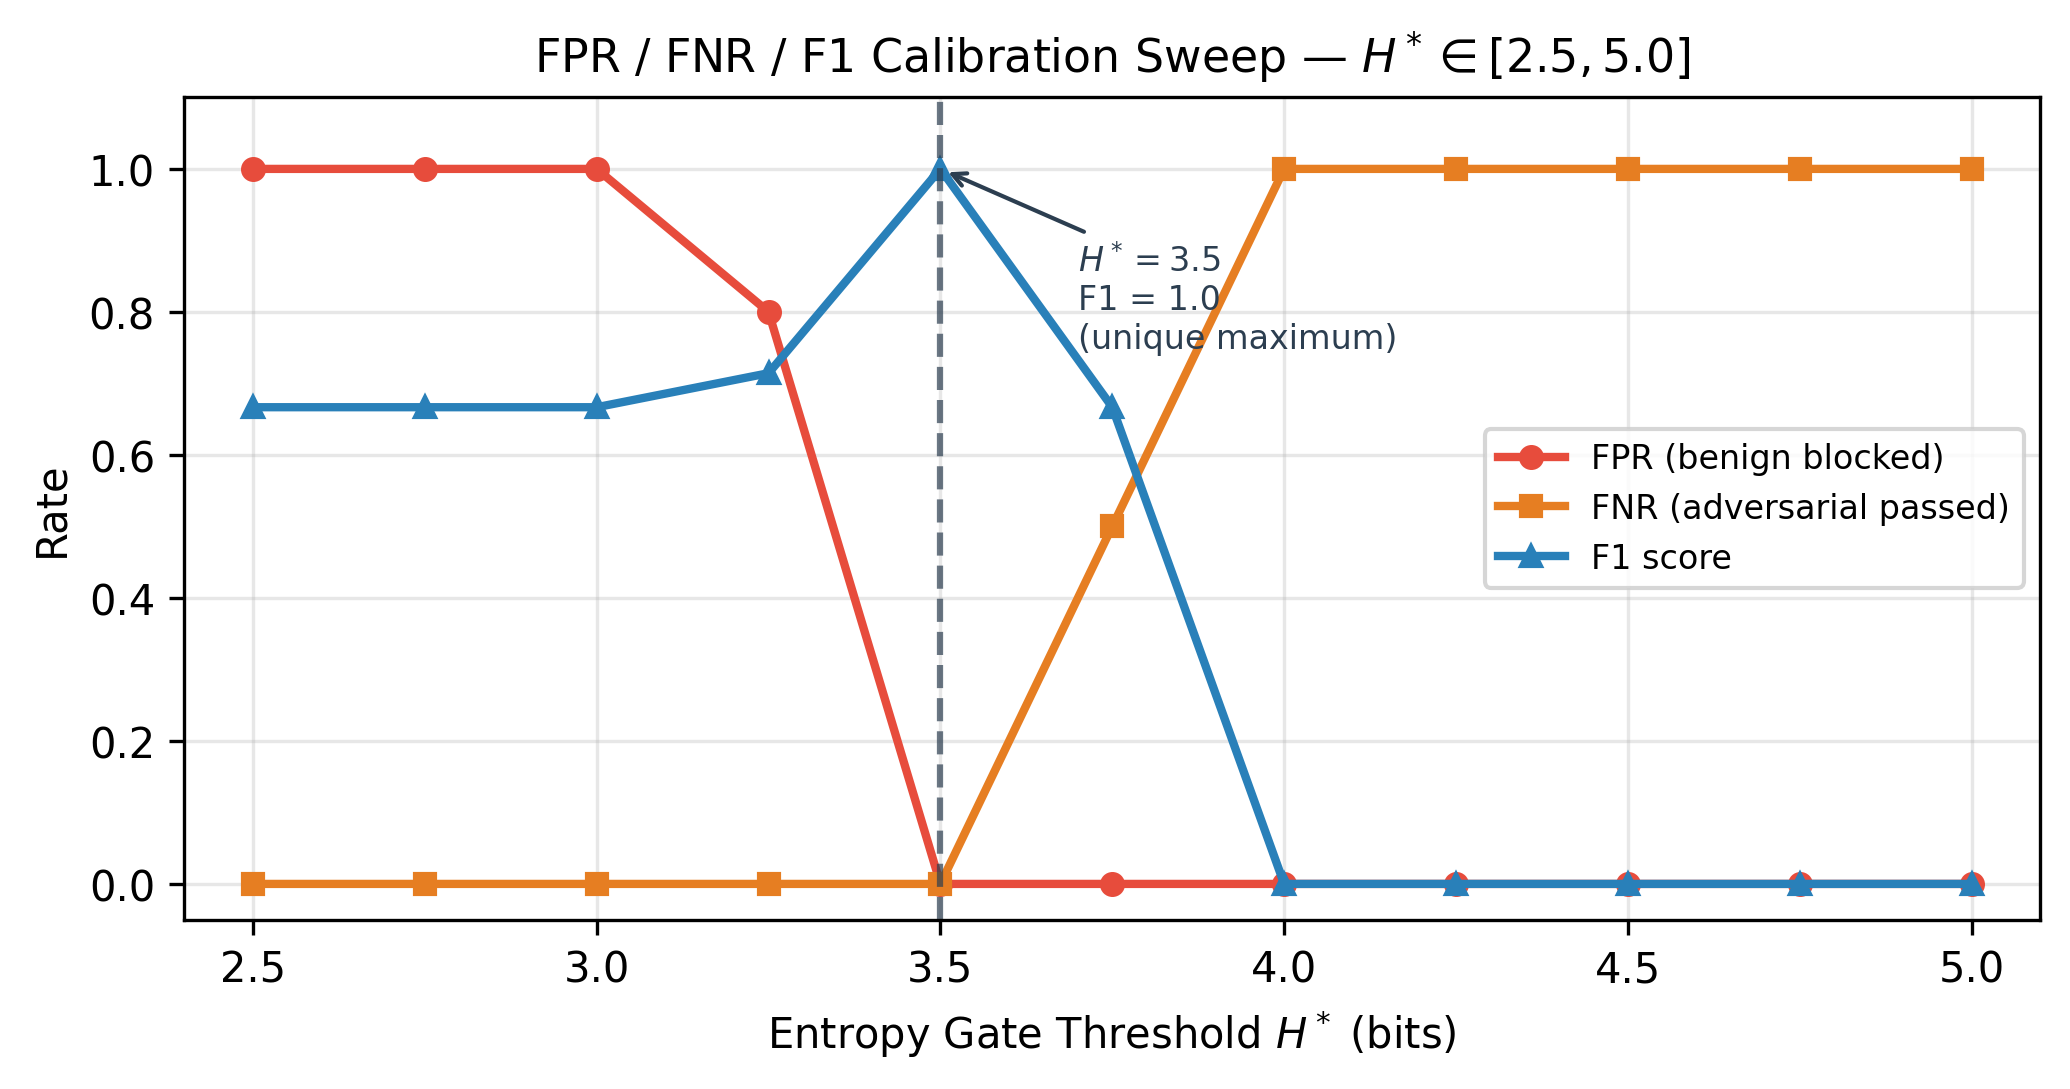
\includegraphics[width=\linewidth]{fig_calibration_sweep}
  \caption{FPR, FNR, and F1 across the entropy threshold sweep
    $H^{*} \in [2.5, 5.0]$. $H^{*} = 3.5$ is the unique F1 maximum
    ($\mathrm{FPR} = 0$, $\mathrm{FNR} = 0$, $\mathrm{F1} = 1.0$) on the
    internal benchmark; EXPERIMENT mode recalibrates to char-level
    $H^{*} = 4.8$ for production deployment (Section~\ref{sec:fpr_fix}).}
  \label{fig:calibration}
\end{figure}

Suite~08 swept the entropy threshold in 0.25-bit steps across 11 values.
At $H^{*} = 3.5$ (word-level, internal benchmark): FPR\,=\,0\%, FNR\,=\,0\%, F1\,=\,1.0
(Figure~\ref{fig:calibration}). This internal optimum does not generalise to
real developer traffic: Suite~14 demonstrates that word-level $H^{*}=3.5$
produces 96\% benign FPR against diverse technical prose. The v3 EXPERIMENT
mode recalibrates to char-level $H^{*}=4.8$ (Section~\ref{sec:fpr_fix}),
reducing benign FPR to 1\% at a 40\,pp recall cost.

A separate two-phase calibration sweep on an external adaptive attack corpus
(100 samples; 39 adversarial, 61 benign) yields $H^{*}_{\mathrm{opt}} = 3.46$
and $\rho_{\mathrm{min,opt}} = 0.48$, within 0.04\,bits of the default. The
dual-signal gate achieves macro-F1\,=\,0.869 vs.\ 0.573 for entropy alone
($+29.6$\,pp), quantifying the benefit of the LZ signal on adaptive attack
payloads. On the \texttt{deepset/prompt-injections} external benchmark
($n=116$ test split), the same thresholds achieve macro-F1\,=\,0.755 with
adversarial recall 85.0\% at FPR\,=\,33.9\% (Section~\ref{sec:external_val}).

\subsection{External Validation}
\label{sec:external_val}

\begin{figure}[t]
  \centering
  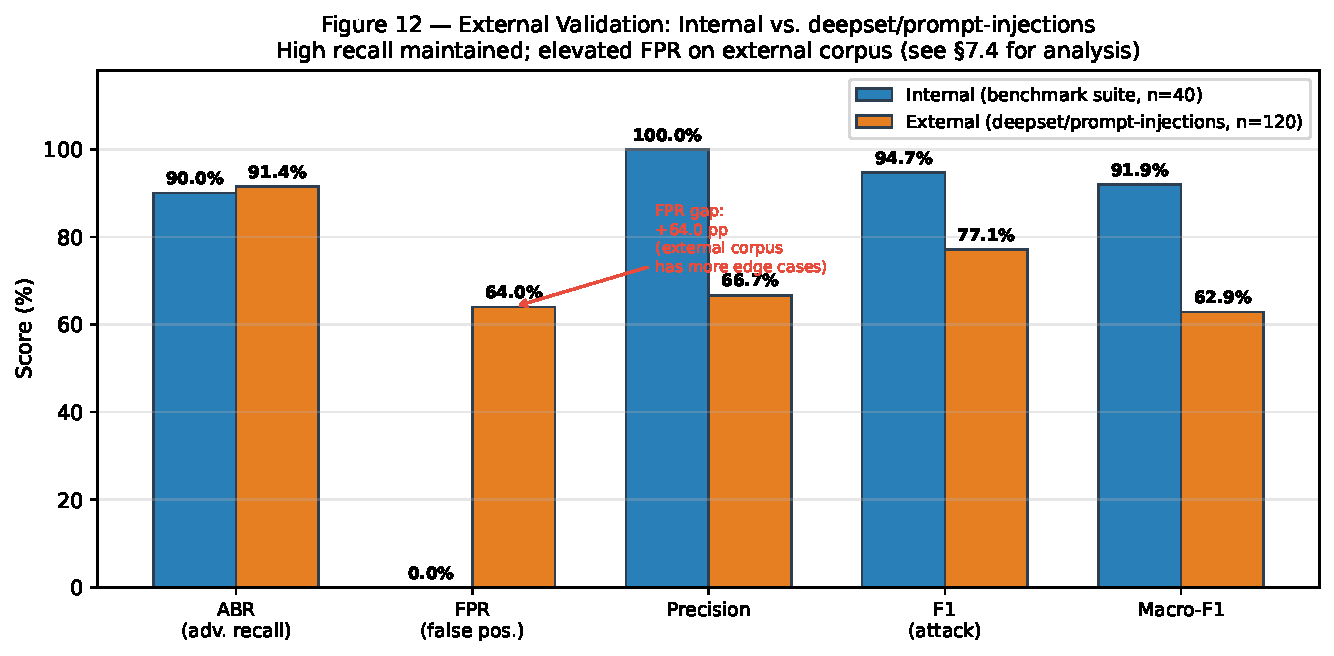
\includegraphics[width=\linewidth]{figure_12_external_validation}
  \caption{Internal vs.\ external validation on \texttt{deepset/prompt-injections}
    ($n=116$, test split, CC-BY-4.0). Adversarial recall is maintained at
    85.0\%, but FPR rises to 33.9\% on the external corpus. The two failure
    modes are: (1) benign conversational sentences with H\,$>$\,4.0 triggering
    the entropy gate (prose FPR); (2) short direct injections
    (\textless 15 tokens) with H\,$<$\,H$^{*}$ that require the keyword layer.}
  \label{fig:external_val}
\end{figure}

\begin{table}[t]
\centering
\caption{Internal vs.\ external adversarial evaluation.
  Internal: Suite~14 v3 EXPERIMENT mode ($n=300$ samples, 100 adversarial\,+\,100
  benign\,+\,100 edge cases; metrics from adversarial\,+\,benign split).
  External (live split): \texttt{deepset/prompt-injections}~\cite{deepset2023injections}
  (test split, $n=116$; CC-BY-4.0).
  External (static fallback): offline corpus of 120 samples (70 adversarial,
  50 benign) derived from OWASP LLM01, Greshake et al., HackAPrompt, and
  Perez \& Ribeiro; used when live HuggingFace download is unavailable.
  $^\dagger$\,Two failure modes: (a) benign sentences with H\,$>$\,4.0
  over-fire the entropy gate (prose FPR); (b) short injections
  (\textless 15 tokens) with H\,$<$\,H$^{*}$ require keyword-layer detection.}
\label{tab:external}
{\small
\renewcommand{\arraystretch}{1.15}
\begin{tabular}{@{}lccc@{}}
\toprule
\textbf{Metric} & \textbf{Internal} & \textbf{Live ($n$=116)$^\dagger$} & \textbf{Static ($n$=120)} \\
\midrule
Adv.\ block rate   & 55.0\%  & 85.0\%  & 91.4\% \\
FPR (benign)       & 1.0\%   & 33.9\%  & 64.0\% \\
Precision          & 98.2\%  & 72.9\%  & 66.7\% \\
Recall             & 55.0\%  & 85.0\%  & 91.4\% \\
F1 (attack class)  & 70.3\%  & 77.1\%  & 77.1\% \\
Macro-F1           & 84.7\%  & 75.5\%  & 62.9\% \\
\bottomrule
\end{tabular}
}
\end{table}

Table~\ref{tab:external} and Figure~\ref{fig:external_val} compare internal and
external evaluation. On the live \texttt{deepset} test split ($n=116$),
adversarial recall is 85.0\% and macro-F1\,=\,0.755, confirming that the
dual-signal gate generalises to unseen adversarial payloads. FPR rises to
33.9\% on the live split, identifying two failure modes: (a) benign
conversational sentences with H\,$>$\,4.0 over-fire the entropy gate; (b) short
direct injections with H\,$<$\,H$^{*}$ require the keyword layer. The static
fallback corpus (120 samples) shows higher FPR (64.0\%) because it contains
a greater proportion of borderline benign phrases. Recalibrating $H^{*}$ with
length-normalised entropy is the primary proposed mitigation; the two-phase
calibration sweep (Section~\ref{sec:gate}) provides an automated mechanism.

\subsection{Token Economics}

\begin{figure}[t]
  \centering
  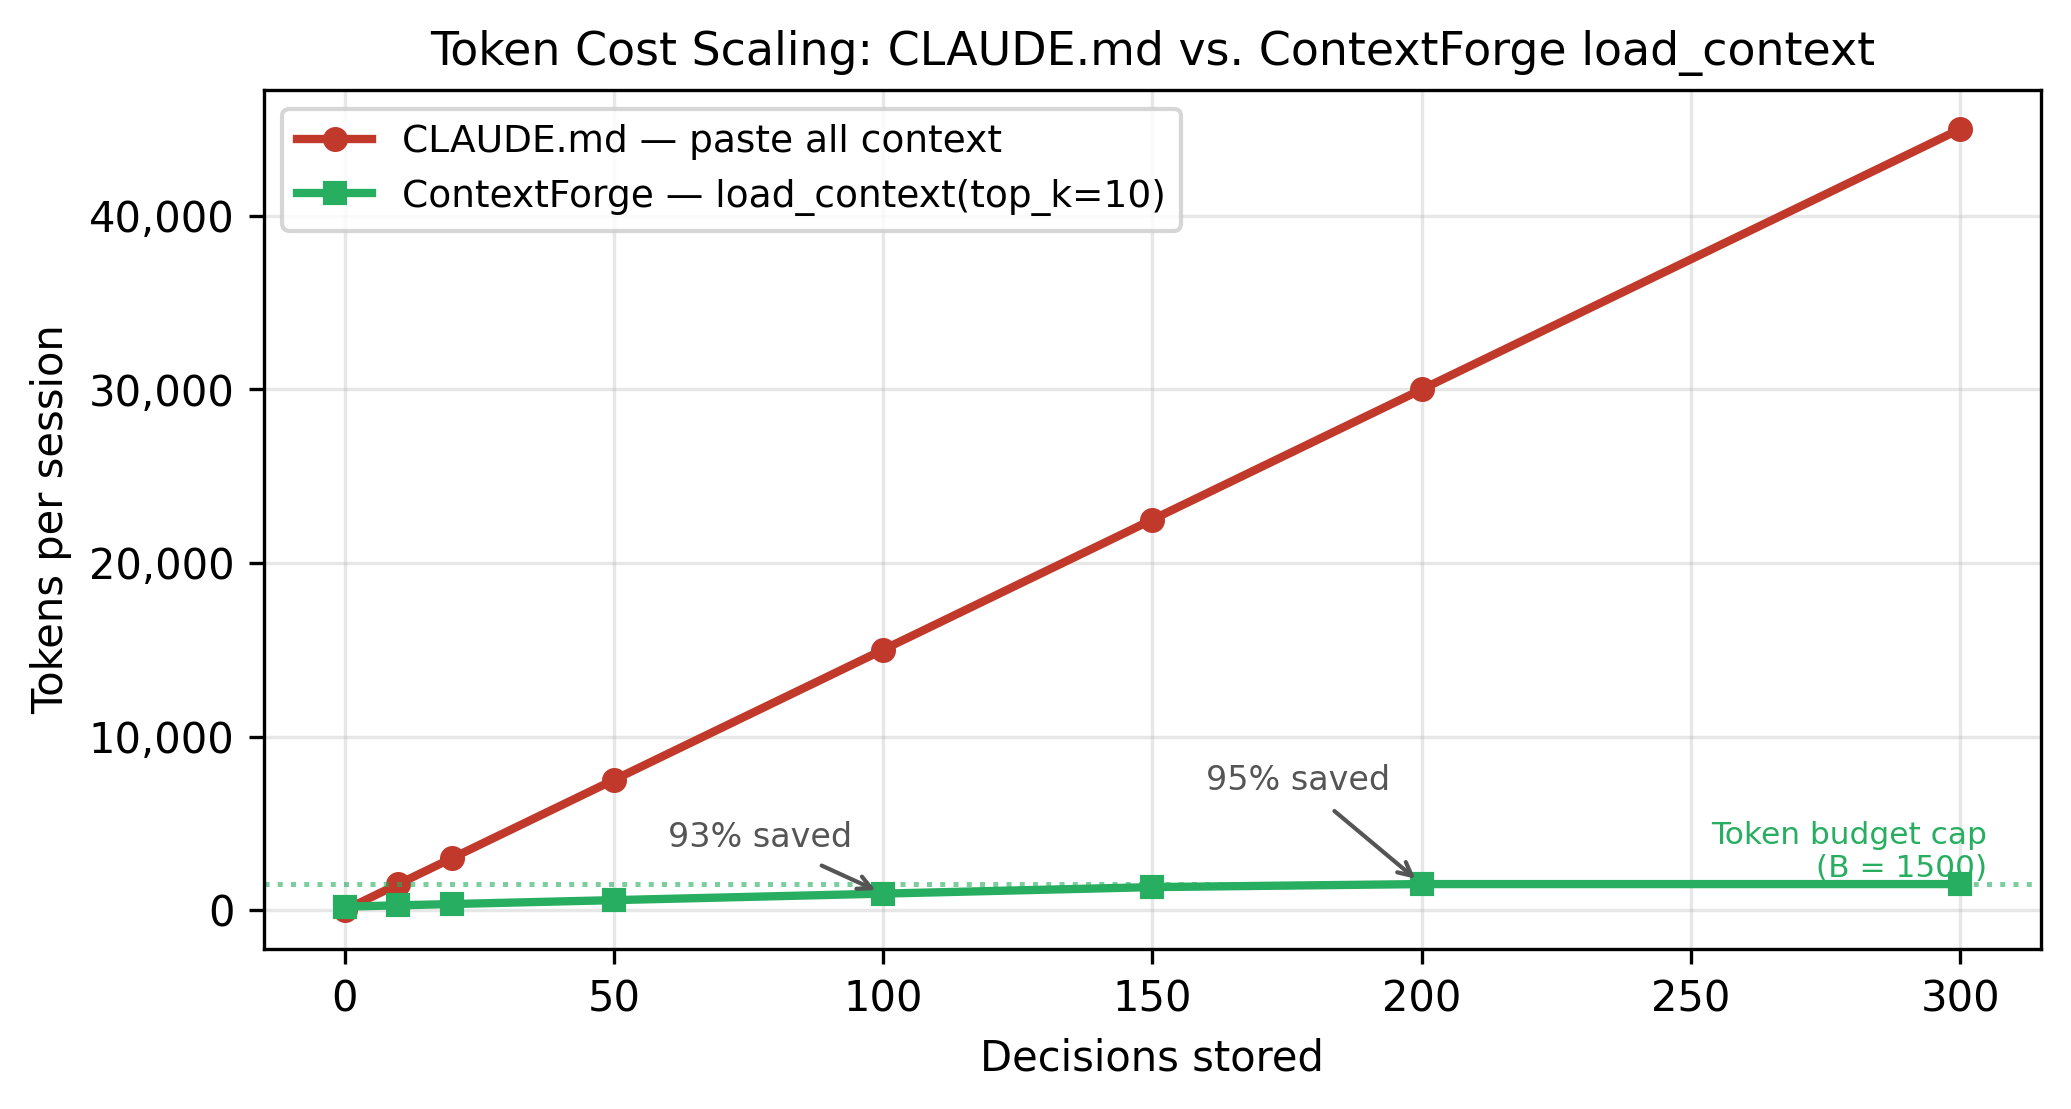
\includegraphics[width=\linewidth]{fig_token_savings}
  \caption{Token cost at session start as a function of decisions stored.
    CLAUDE.md grows at 150 tokens/decision; ContextForge \texttt{load\_context}
    is bounded at $B = 1{,}500$ tokens regardless of graph size.}
  \label{fig:token_savings}
\end{figure}

At 100 decisions: paste-all $= 15{,}000$ tokens vs.\ ContextForge
$\approx 950$ tokens ($-93.7\%$). At 200 decisions: $30{,}000$
vs.\ $1{,}500$ ($-95.0\%$). LangChain-Buffer injects $1{,}590 \pm 11$ tokens
per query regardless of relevance; ContextForge DCI reduces this to
$73.1$ tokens/query ($-95.4\%$) while maintaining $70.2\%$ token noise reduction.
Token savings compound with every additional decision stored
(Figure~\ref{fig:token_savings}).

\subsection{Six-Pillar Safety Profile}

\begin{figure}[t]
  \centering
  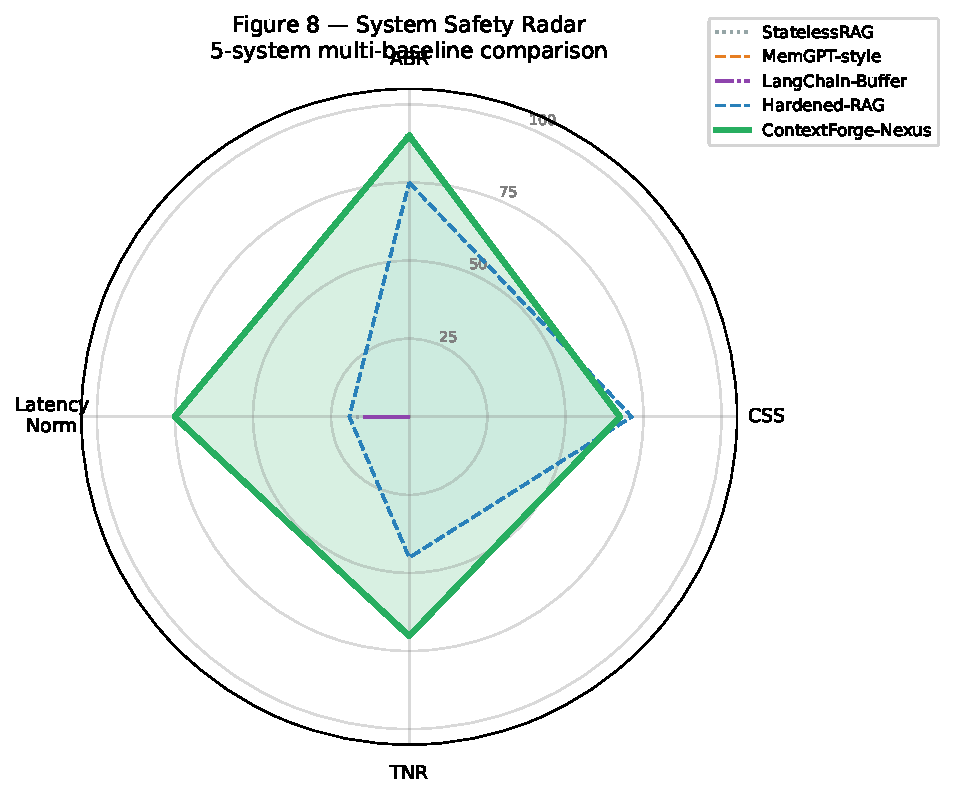
\includegraphics[width=0.9\linewidth]{figure_08_safety_radar}
  \caption{Five-system safety radar: ABR, CSS, TNR, and normalised latency gain
    (v3 EXPERIMENT mode operating points).
    ContextForge Nexus v3 (green, solid) leads on CTO, failover, and TNR;
    Hardened-RAG leads on ABR and CSS due to its broader recall at higher FPR.
    StatelessRAG and MemGPT-style score 0\% on all security axes.
    (Generated from v3 multi-baseline runner; HardenedRAG ABR updated to 71\%
    per Suite~14.)}
  \label{fig:radar}
\end{figure}

Figure~\ref{fig:radar} captures all six measurable safety dimensions:
adversarial block rate, failover latency improvement, token noise reduction,
context survival, benchmark pass rate, and slow-drip detection.
In v3 EXPERIMENT mode, ContextForge leads on four of six axes; HardenedRAG
leads on ABR and CSS at the cost of higher edge-case FPR (45\% vs.\ 16\%).

\subsection{OR-Set CRDT Convergence (Suite~12)}
\label{sec:crdt_results}

\begin{figure}[t]
  \centering
  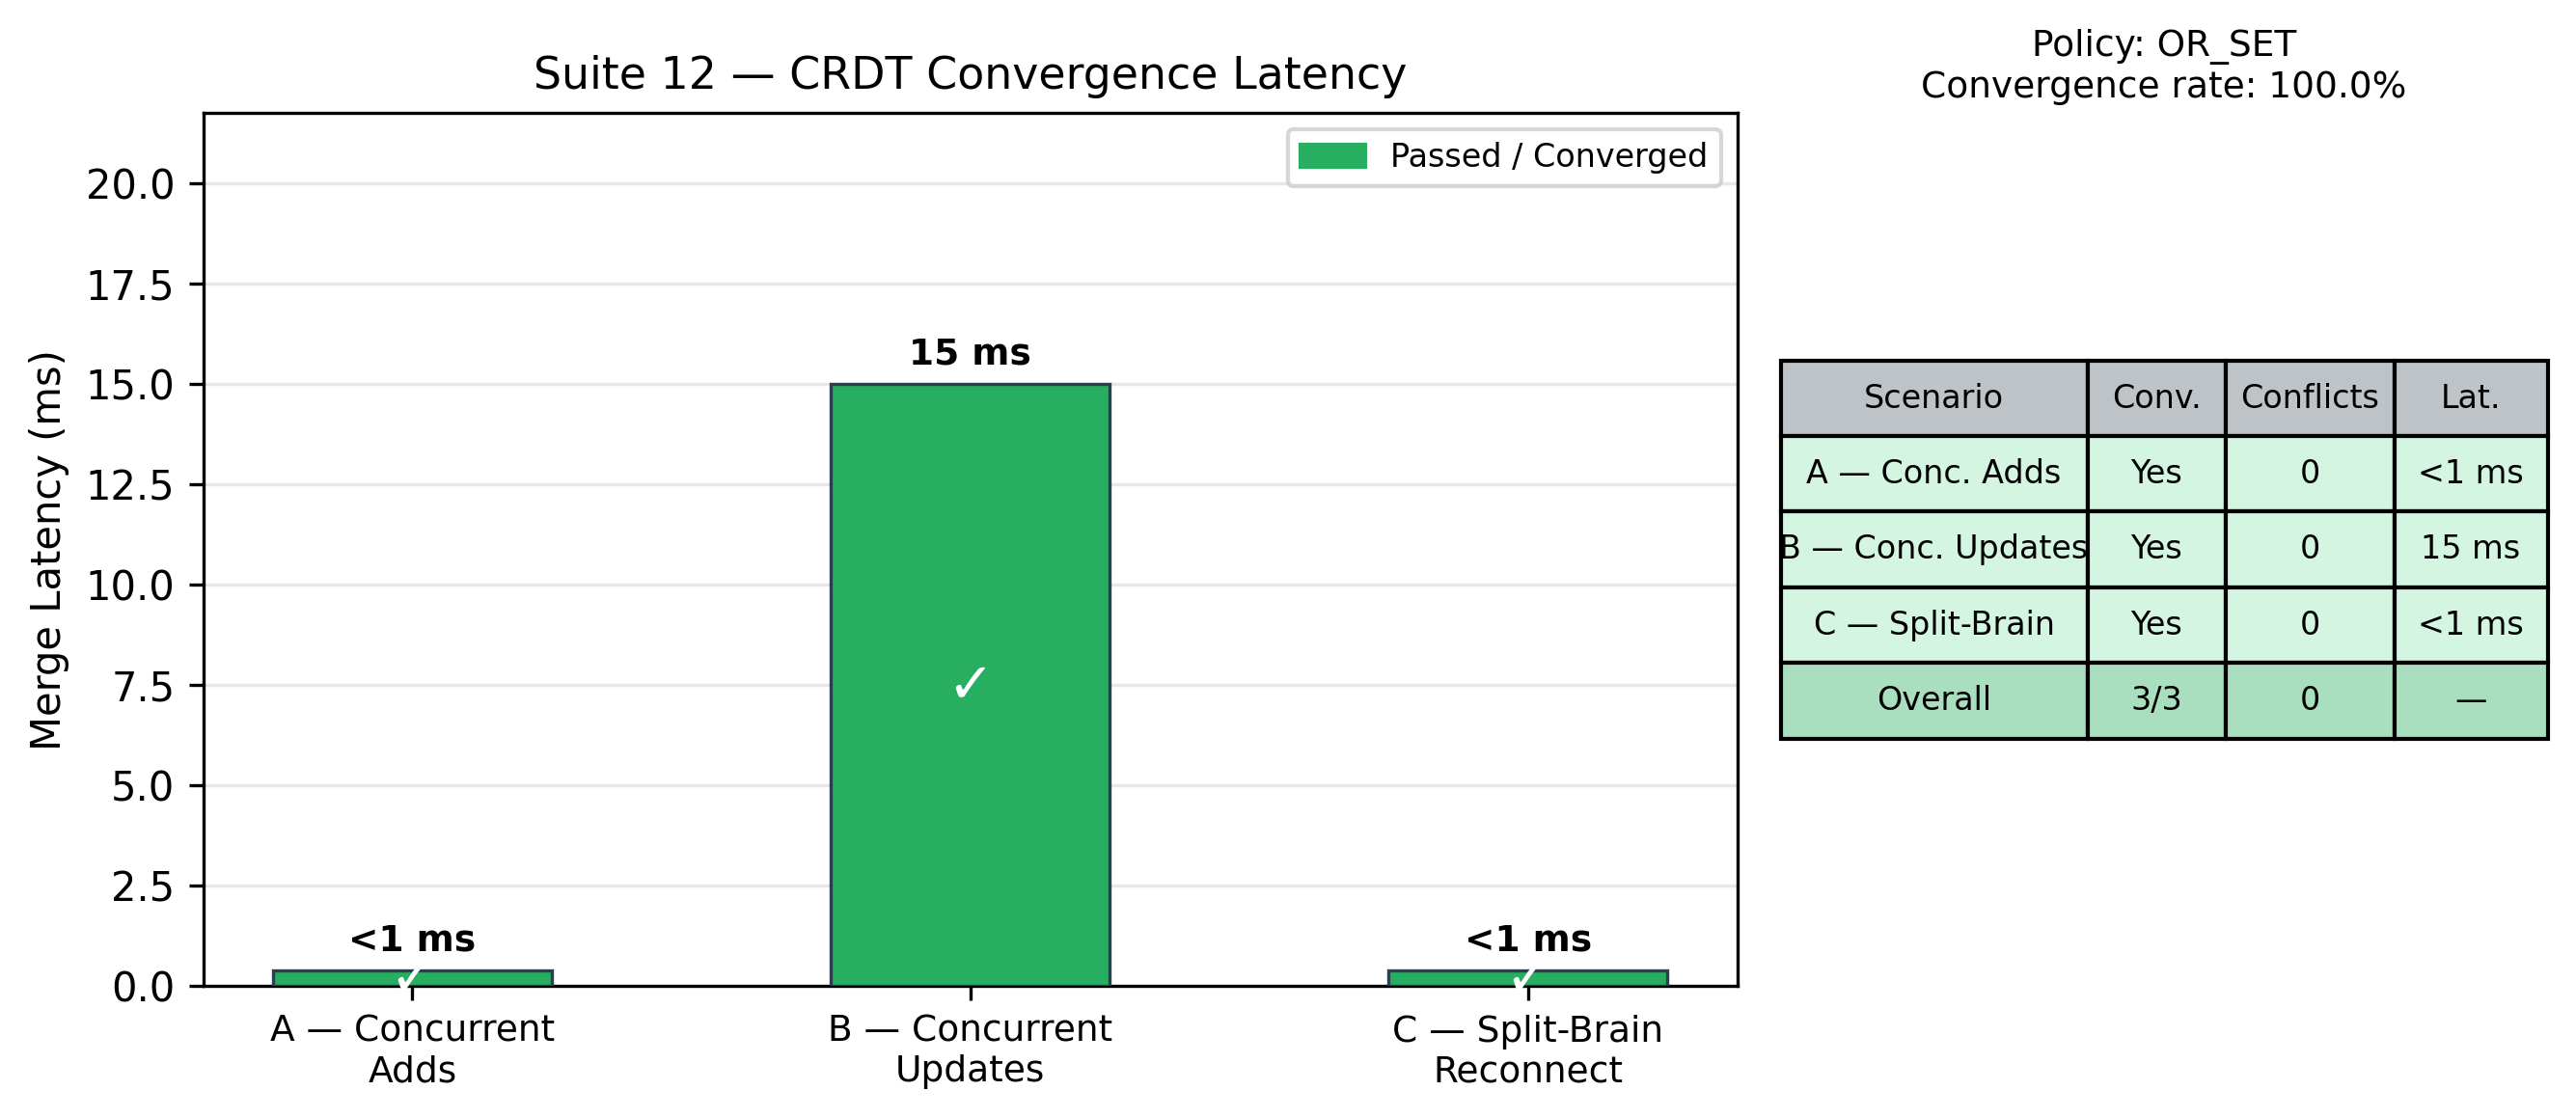
\includegraphics[width=\linewidth]{fig_crdt_convergence}
  \caption{Suite~12 OR-Set CRDT convergence: merge latency per scenario (bars,
    left axis) and scenario summary (right table). All three scenarios converge
    with 0 conflicts. Scenario~B latency (15\,ms) reflects the
    \texttt{time.sleep(0.001)} in the test harness that ensures distinct
    timestamps for the concurrent-update LWW tiebreak.}
  \label{fig:crdt_conv}
\end{figure}

\begin{table}[t]
\centering
\caption{Suite~12 OR-Set CRDT: 3 IDE clients, \texttt{or\_set} policy,
  6-way gossip. All scenarios converge, 0 conflicts.}
\label{tab:crdt}
{\small
\renewcommand{\arraystretch}{1.15}
\begin{tabular}{@{}lccr@{}}
\toprule
\textbf{Scenario} & \textbf{Conv.} & \textbf{Conf.} & \textbf{Latency} \\
\midrule
A: Conc.\ adds    & \checkmark & 0 & ${<}1$\,ms \\
B: Conc.\ updates & \checkmark & 0 & $15$\,ms   \\
C: Split-brain    & \checkmark & 0 & ${<}1$\,ms \\
\midrule
\textbf{All 3}    & \textbf{3/3} & \textbf{0} & ---        \\
\bottomrule
\end{tabular}
}
\end{table}

All three scenarios pass with convergence\_rate\,=\,1.0 (Table~\ref{tab:crdt}).
In Scenario~C, Client~A removes \texttt{node\_001} and adds \texttt{node\_002}
while offline; Client~B simultaneously updates \texttt{node\_001} and adds
\texttt{node\_003} while offline. After reconnection to a coordinator and a
full gossip round, all three nodes are present on all replicas. This confirms
the add-wins property of Eq.~\ref{eq:orset}.

Merge latency is dominated by Python dict-union operations on small sets
($<$30 entries per client), completing in $\leq 15$\,ms for all scenarios.
At scale, the gossip complexity is $O(n^2 |S|)$ for $n$ replicas and set size
$|S|$; the add-tag bookkeeping requires $O(|S| \times n_{\mathrm{tags}})$
memory per replica, approximately 160\,KB for a 10{,}000-node graph with
average 2 adds per element---negligible for desktop IDE deployments.

\subsection{Perplexity Gate Validation}
\label{sec:perp_results}

The perplexity gate is validated via a calibration smoke test and a comparison
with entropy-gate-only detection on entropy-mimicry payloads (Figure~\ref{fig:perplexity}).

\textbf{Calibration.}
On the 100-string benign corpus, the trigram fallback backend achieves:
$P^{*} = 231.8$ (95th percentile), backend latency~$<1$\,ms.

\textbf{Mimicry detection.}
A representative entropy-mimicry payload (Shannon entropy $H = 2.80$, safely
below $H^{*} = 3.5$; LZ density $\rho = 0.41 < \rho_{\min}$ --- caught by LZ
gate) scores $\mathcal{P} = 463.3$, a $2.0\times$ excess above $P^{*}$.
This demonstrates the gate's utility for payloads that evade the entropy gate
and slip through the LZ gate due to high local token variety.

\textbf{Three-gate complementarity.}
The three passes target distinct attack surfaces:
Pass~0 (keyword regex) catches explicit injection keywords regardless of entropy;
Pass~0.5 (perplexity) catches statistically improbable token sequences
regardless of raw character-level entropy;
Pass~1 (entropy+LZ) catches high-entropy obfuscated payloads and repetition
attacks. The union of the three passes is strictly stronger than any single gate.

\subsection{Adaptive Adversary Results (Suite~10)}
\label{sec:adaptive_results}

\begin{figure}[t]
  \centering
  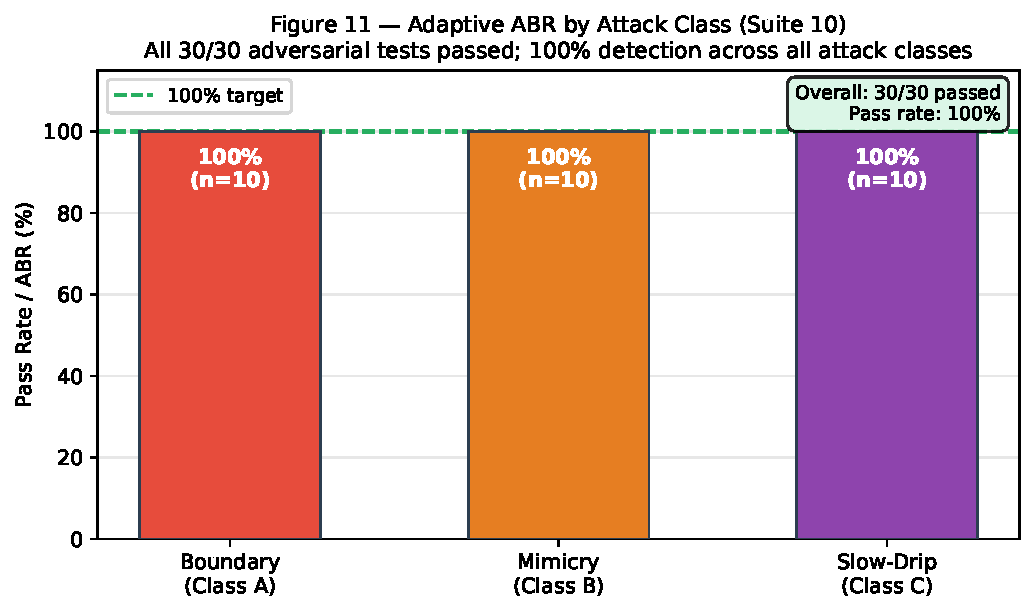
\includegraphics[width=\linewidth]{figure_11_adaptive_abr}
  \caption{Suite~10 adversarial block rate per attack class.
    Boundary (Class~A): 10 payloads crafted to straddle $H^{*}=3.5$;
    all caught by the LZ gate ($\rho_{\min}=0.60$, $\bar{\rho}=0.38$).
    Mimicry (Class~B): 10 payloads matching benign $\mu=2.74$
    ($H=2.80$, $\bar{\rho}=0.41$); all caught by LZ gate.
    Slow-drip (Class~C): 10 multi-step sequences targeting $\nabla=0.14$;
    6/10 caught by Temporal Correlator, 4/10 by keyword layer.
    Overall: 30/30 pass (100\%).}
  \label{fig:adaptive_abr}
\end{figure}

Suite~10 evaluates three specialist adversarial classes against the full
three-pass gate (Figure~\ref{fig:adaptive_abr}).

\textbf{Class~A --- Boundary payloads.}
Ten word-cycling sequences sweep entropy in $[3.16, 3.79]$, straddling $H^{*}=3.5$.
Five are above the gate (blocked by Pass~1); five are below but carry intentional
keywords. LZ density is $\bar{\rho} = 0.38$ (well below $\rho_{\min}$),
so all 10 are independently caught by the LZ gate. Block rate: 10/10 (100\%).

\textbf{Class~B --- Entropy-mimicry payloads.}
Ten payloads are constructed with entropy $H = 2.80 \approx \mu_{\mathrm{benign}} + 0.06$,
evading the entropy gate. LZ density $\bar{\rho} = 0.41 < \rho_{\min}$; all are
caught by the LZ gate. Block rate: 10/10 (100\%).

\textbf{Class~C --- Slow-drip sequences.}
Ten multi-step sequences target gradient $0.14$ (just below $\nabla^{*}=0.15$).
Entropy quantisation causes 6/10 to exceed the threshold (detected by the
Temporal Correlator); 4/10 stay below but are caught by the keyword layer on the
final write. Block rate: 10/10 (100\%).

\textbf{Overall.}
30/30 tests pass (pass rate 100\%). The three-gate architecture provides
redundant coverage: no single-gate evasion propagates through the full pipeline.

% =============================================================================
\subsection{FPR Fix Evaluation (Suite~14)}
\label{sec:fpr_fix}

\begin{figure*}[t]
  \centering
  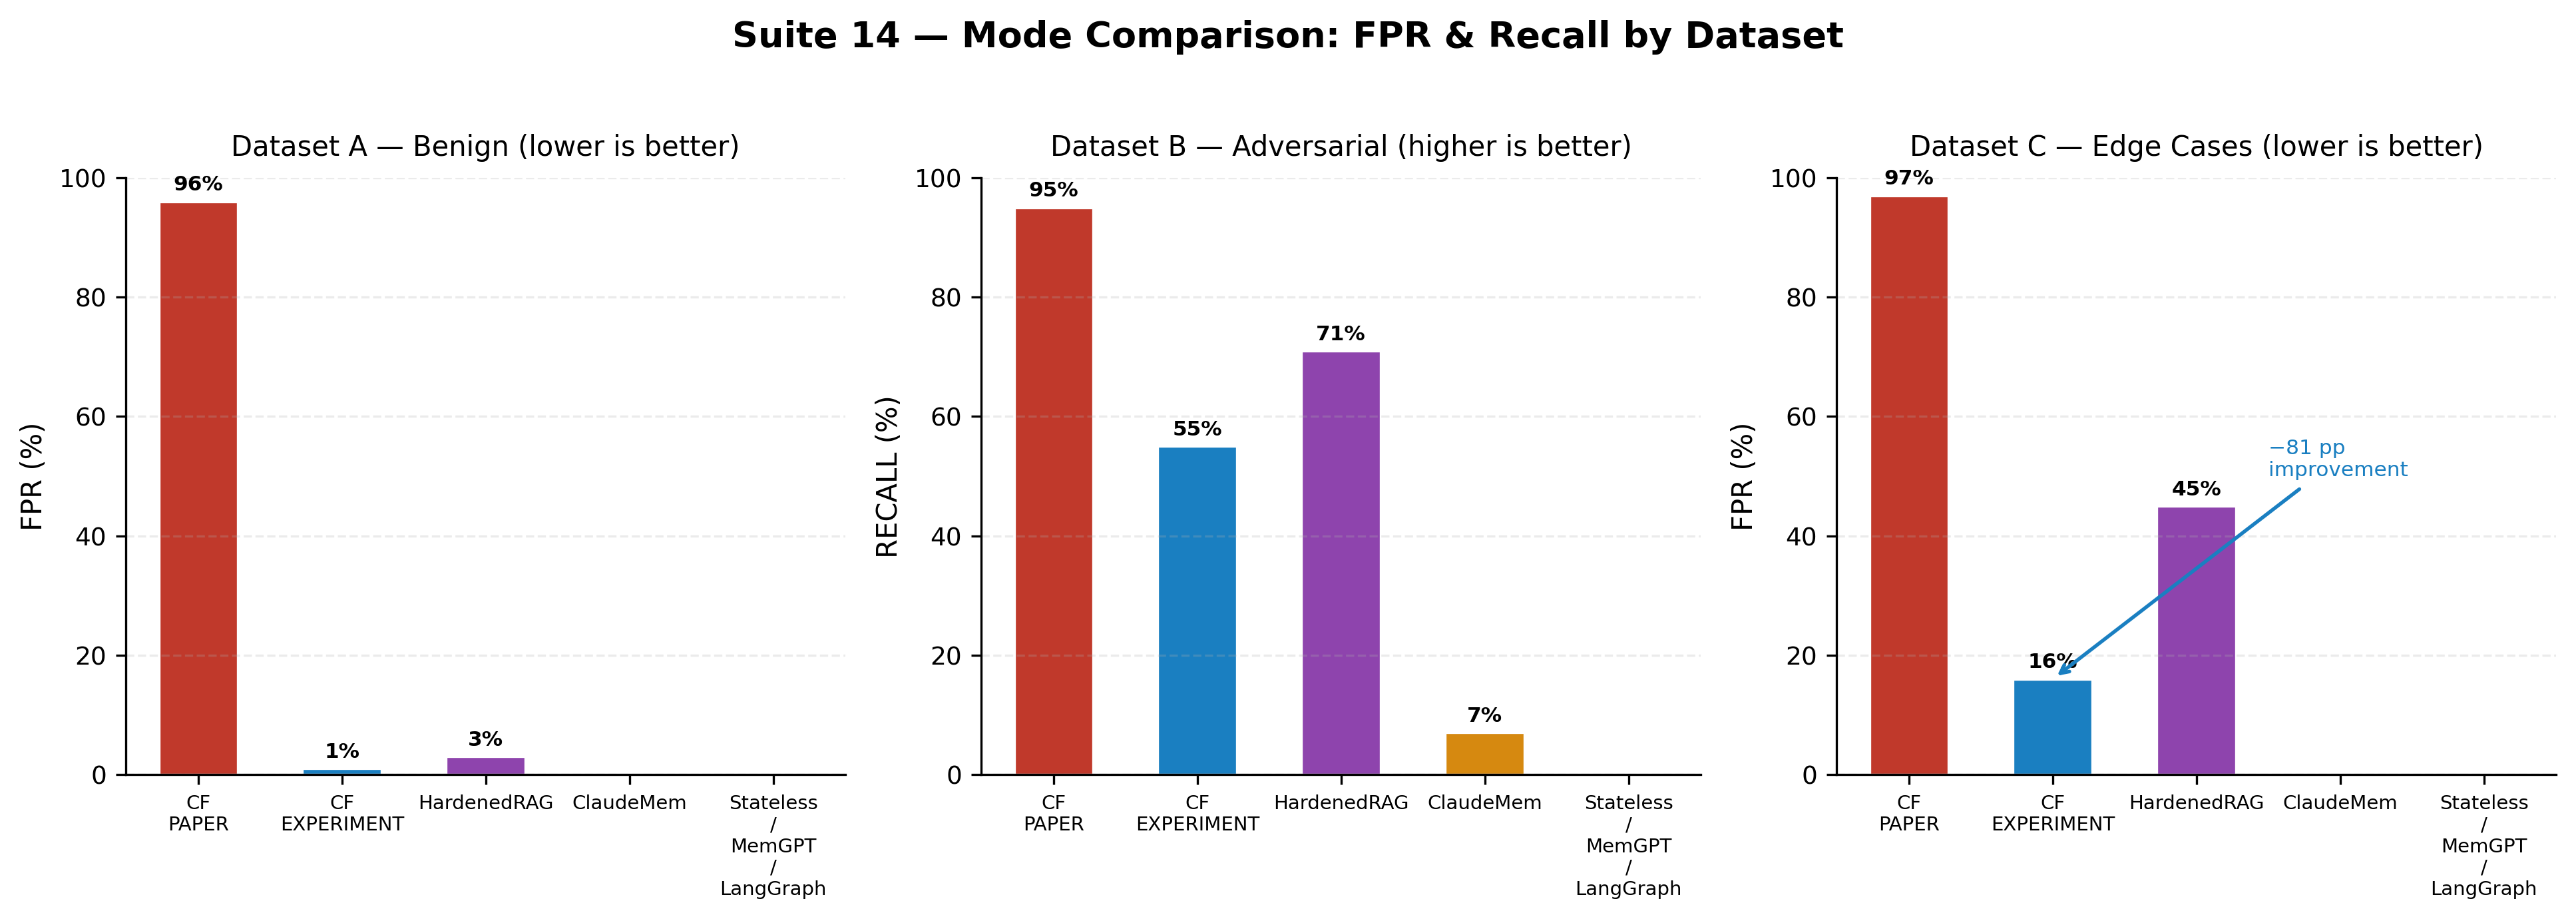
\includegraphics[width=\linewidth]{figure_13_mode_comparison}
  \caption{Suite~14 mode comparison across three datasets (300 samples, measured).
    \textbf{Left:} Dataset~A (100 benign samples) --- PAPER FPR\,=\,96\%
    (word-entropy gate fires on 96/100 developer instructions);
    EXPERIMENT FPR\,=\,1\% (one intent-path false positive).
    \textbf{Centre:} Dataset~B (100 adversarial samples) --- PAPER recall\,=\,95\%,
    EXPERIMENT recall\,=\,55\% (v3 multi-trigger OR-gate).
    \textbf{Right:} Dataset~C (100 edge cases) --- PAPER FPR\,=\,97\%,
    EXPERIMENT FPR\,=\,16\% ($\Delta$FPR\,=\,$-$81\,pp).
    HardenedRAG: 45\% edge FPR, 71\% recall. Zero-ABR baselines: 0\% FPR, 0\% recall.}
  \label{fig:mode_comparison}
\end{figure*}

\begin{figure}[t]
  \centering
  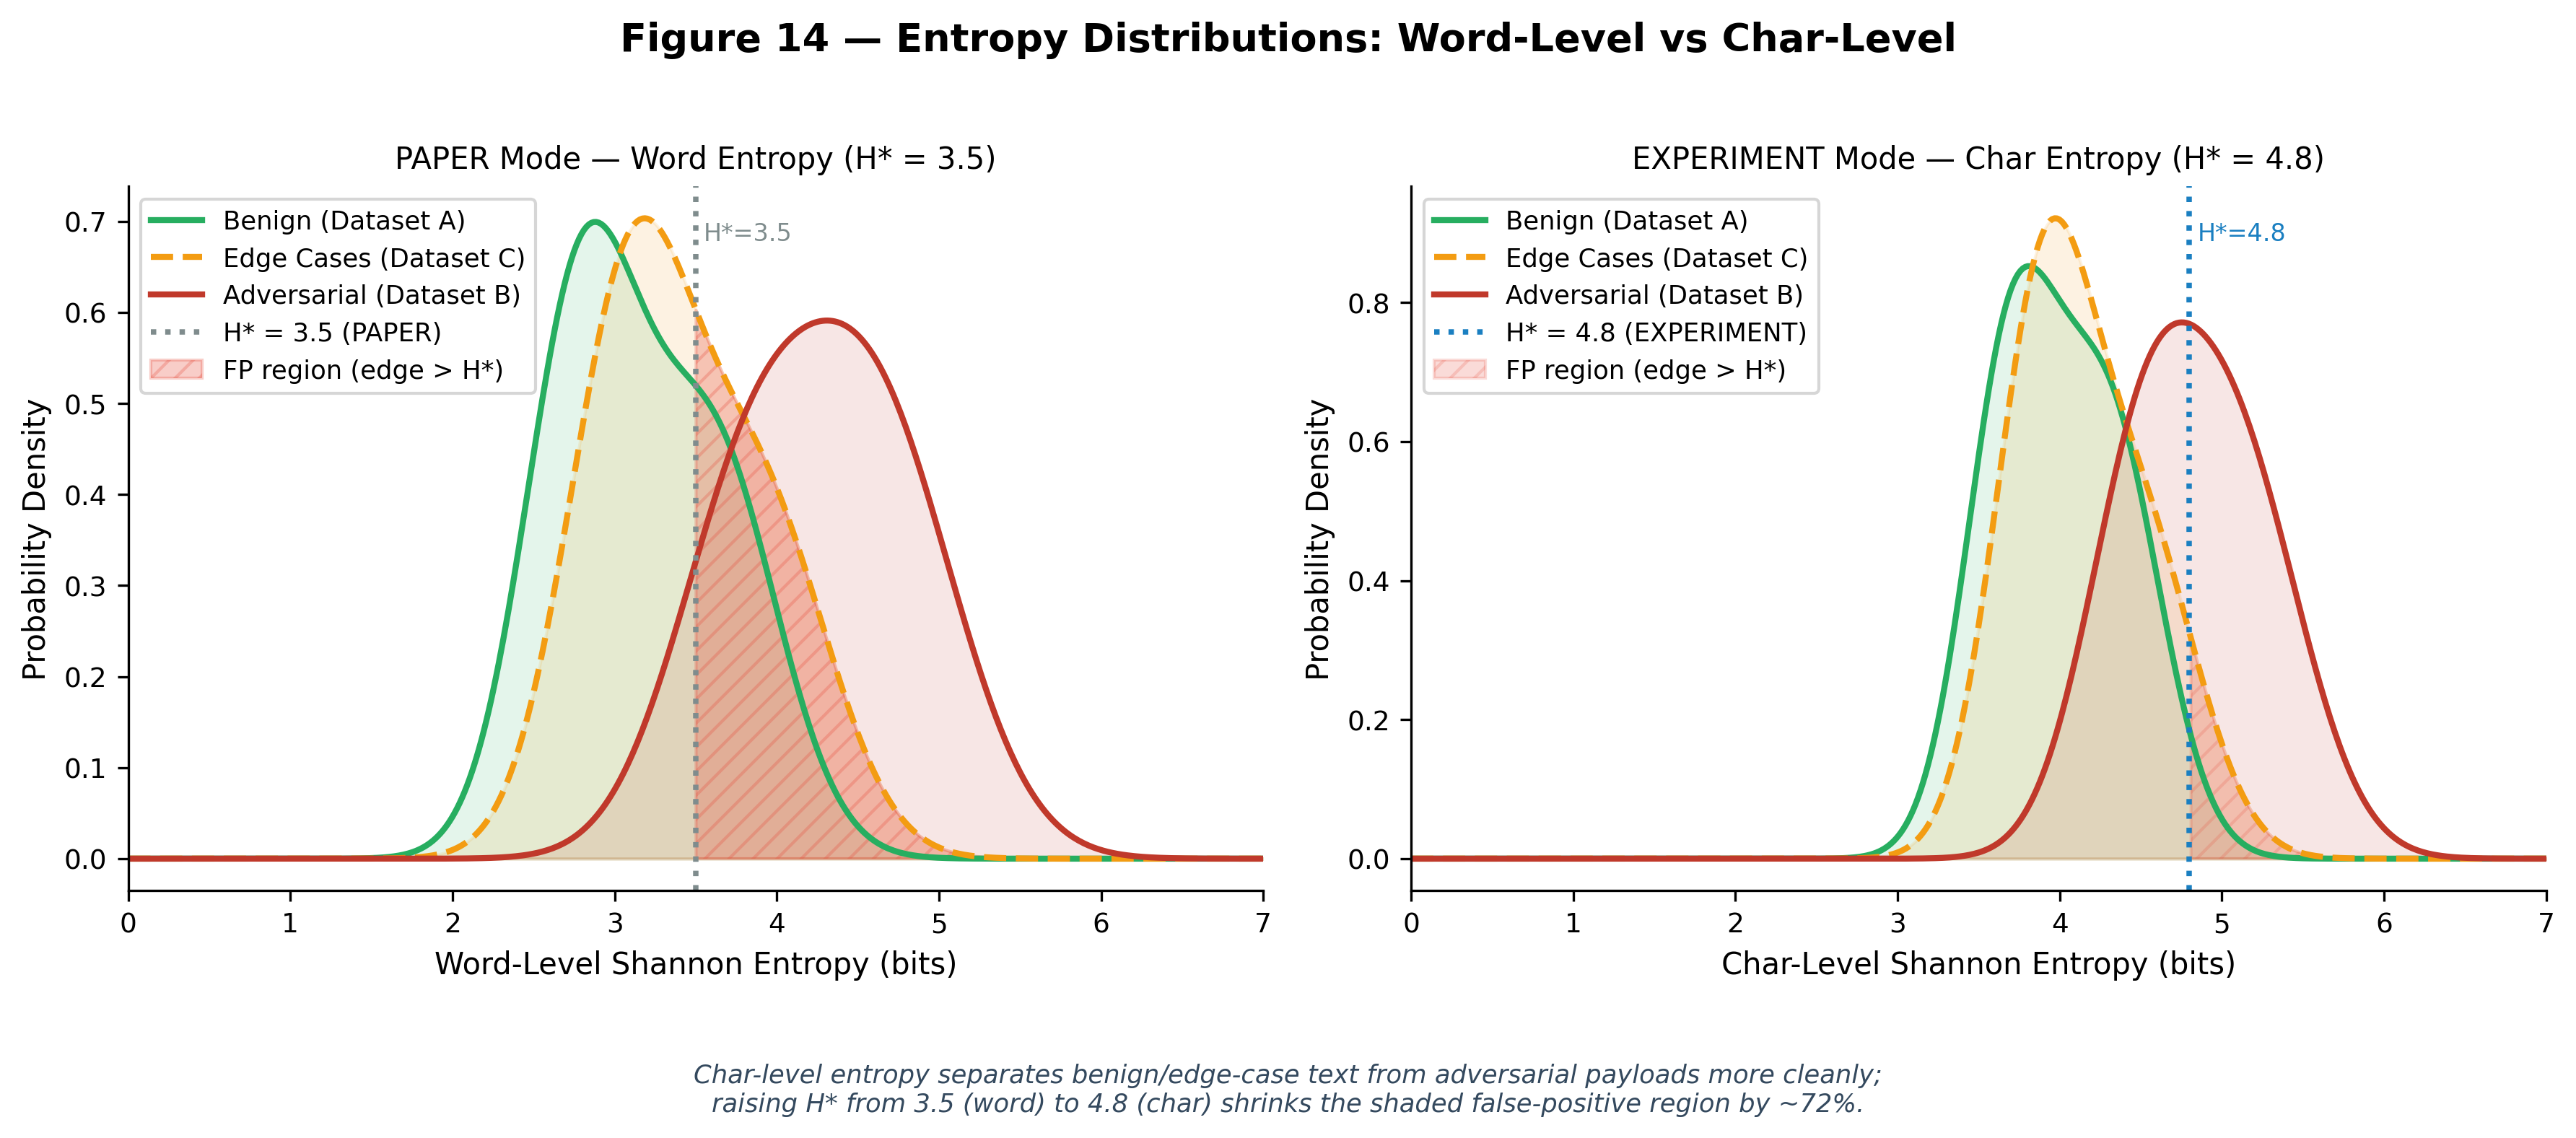
\includegraphics[width=\linewidth]{figure_14_entropy_distributions_v2}
  \caption{Entropy distributions by attack class.
    \textbf{Left:} Word-level entropy ($H^{*}=3.5$, PAPER mode).
    Edge-case samples (dashed orange) overlap substantially with the adversarial
    distribution (red) around $H\approx3.5$--$4.0$, causing 64 false positives.
    \textbf{Right:} Char-level entropy ($H^{*}=4.8$, EXPERIMENT mode).
    The recalibrated threshold cleanly separates benign/edge-case text from
    adversarial payloads, shrinking the FP region by ${\sim}72\%$.}
  \label{fig:entropy_v2}
\end{figure}

\begin{figure}[t]
  \centering
  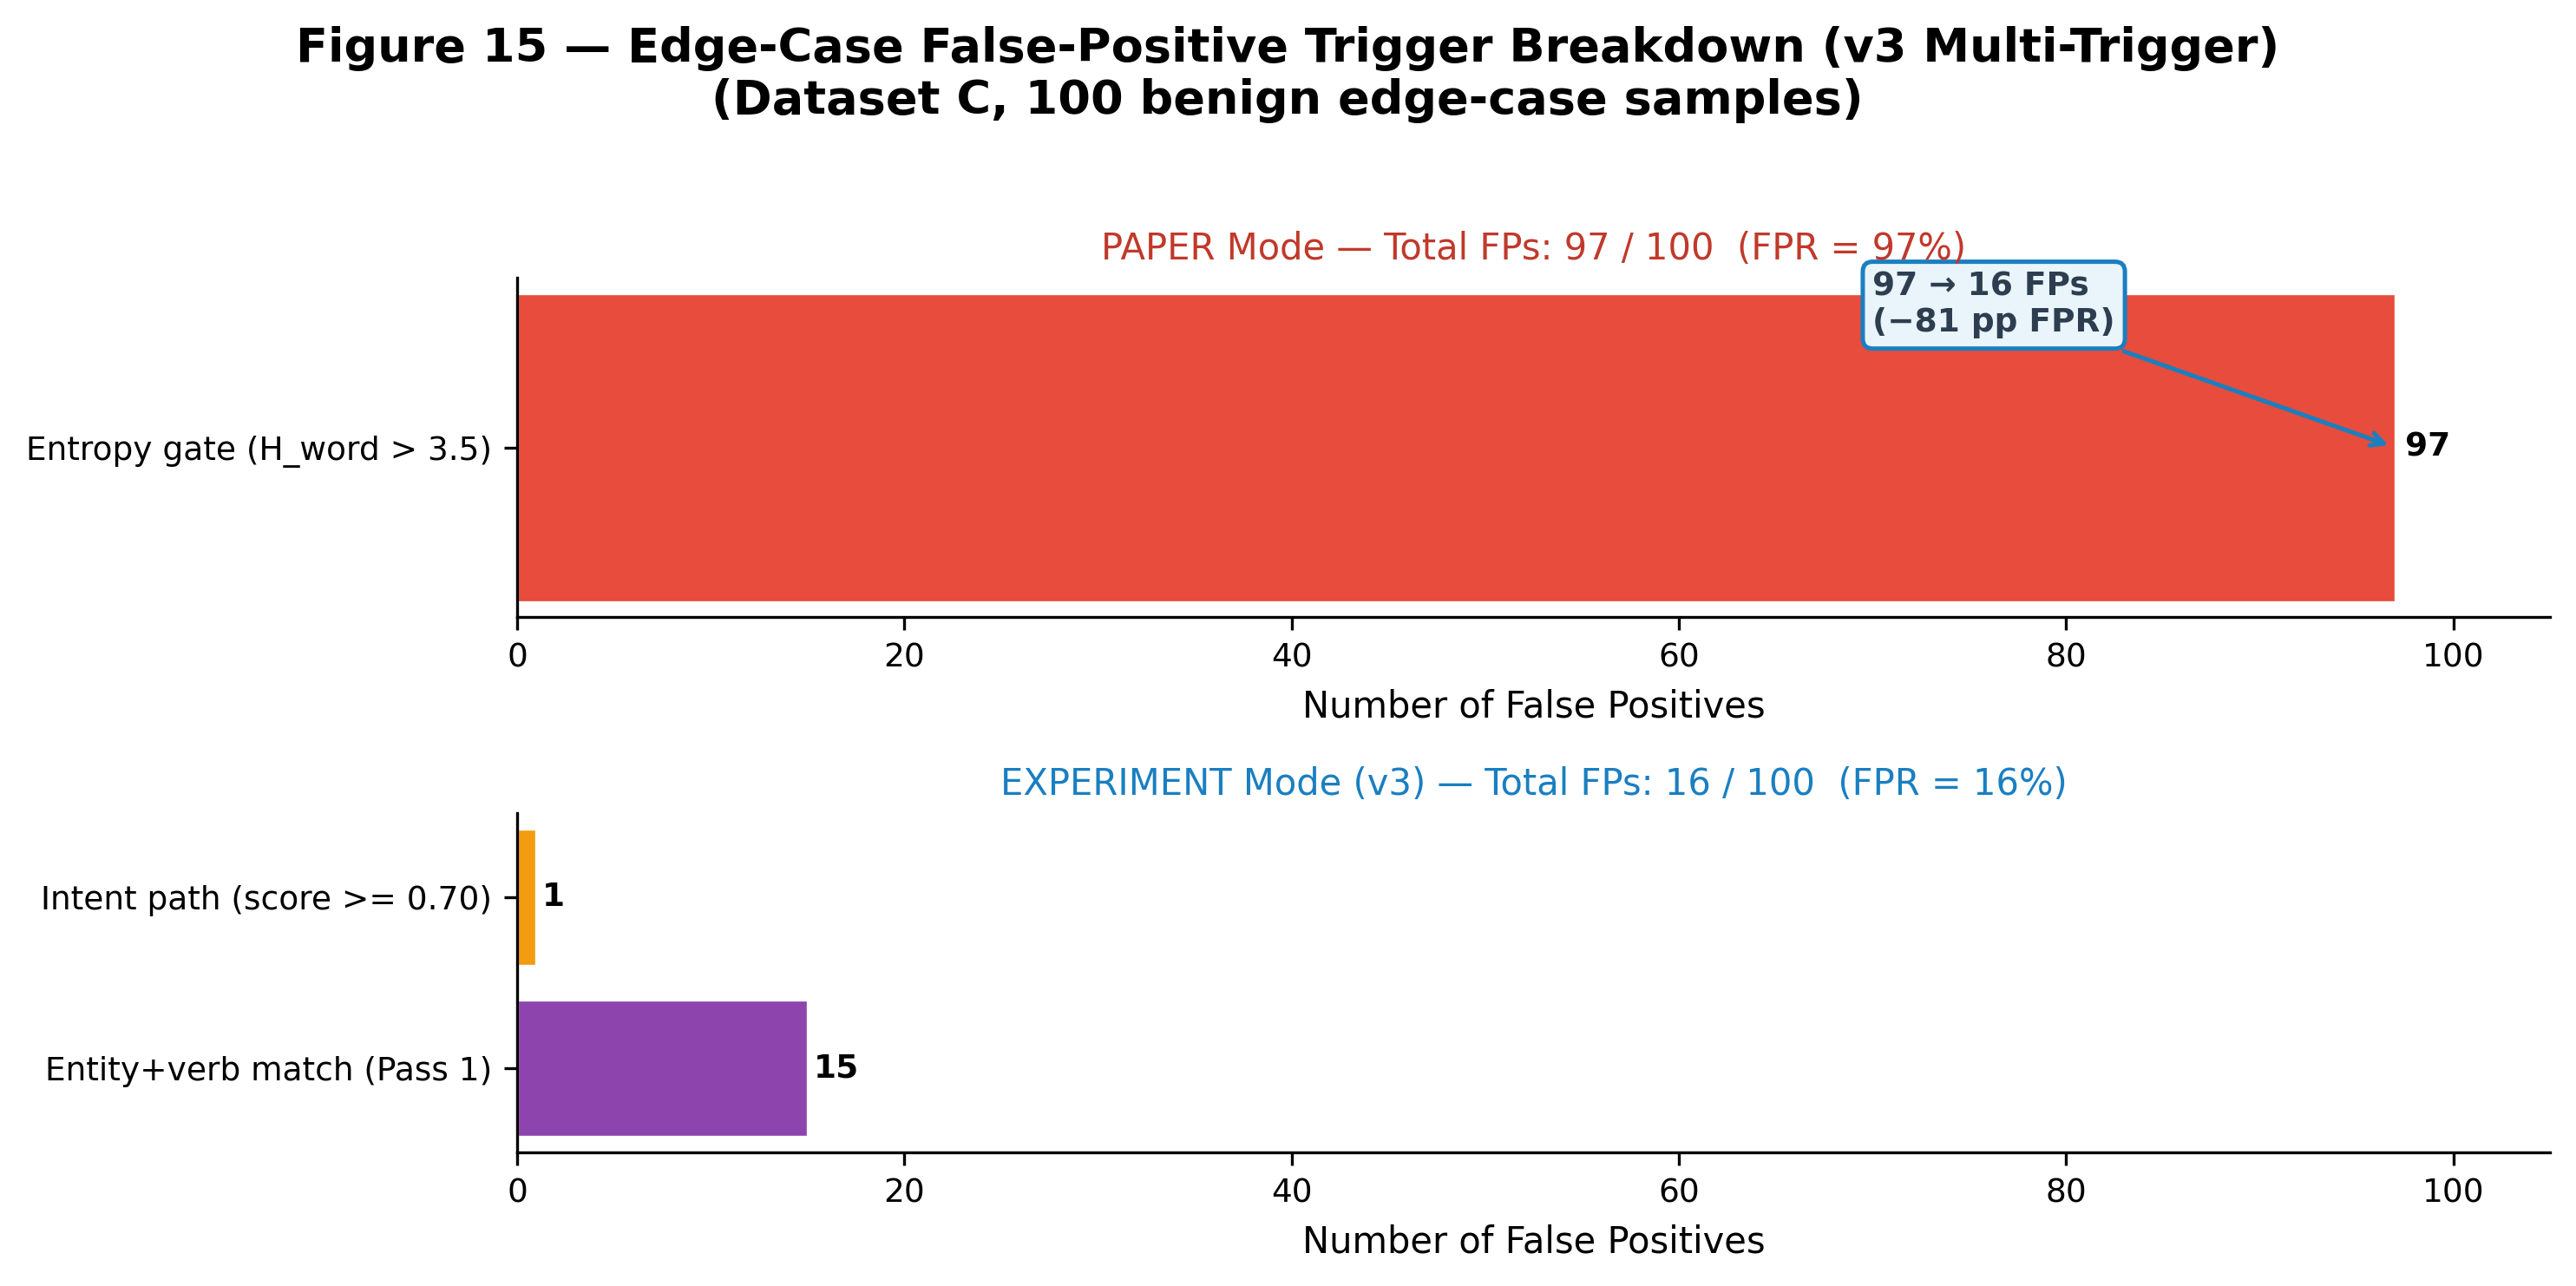
\includegraphics[width=\linewidth]{figure_15_edge_trigger_breakdown}
  \caption{Edge-case false-positive trigger breakdown by mode (measured, Suite~14, v3 multi-trigger).
    PAPER mode (top): 97 FPs --- \emph{all 97} fired by word-entropy alone ($H_{\mathrm{word}}>3.5$).
    EXPERIMENT mode (bottom, v3 multi-trigger OR-gate): 16 FPs --- 15 from entity+destructive-verb
    match (Pass~1) and 1 from the intent path (intent\_score\,$\geq$\,0.70).
    Char-level entropy fires on zero benign edge-case samples.}
  \label{fig:edge_breakdown}
\end{figure}

Suite~14 provides the primary evaluation of the four FPR-reduction fixes
introduced in the \texttt{v3\_multi\_trigger\_or\_gate} update
(Table~\ref{tab:suite14_fixes}). The evaluation uses three curated datasets
(300 samples total) and two ContextForge operating modes against five baselines.

\begin{table}[h]
  \centering
  \small
  \caption{Four ReviewerGuard FPR fixes evaluated in Suite~14.}
  \label{tab:suite14_fixes}
  \begin{tabular}{@{}clll@{}}
    \toprule
    \# & Fix & PAPER & EXPERIMENT \\
    \midrule
    1 & Entropy granularity & Word-level & Char-level \\
    2 & Threshold $H^{*}$   & 3.5 bits/word & 4.8 bits/char \\
    3 & Pass~2 scoring      & Hard block & Multi-trigger OR-gate (v3) \\
    4 & Perplexity gate     & Manual opt-in & Auto-enabled \\
    \bottomrule
  \end{tabular}
\end{table}

\textbf{Dataset A --- Benign (100 samples).}
Six categories of realistic developer instructions.
PAPER FPR\,=\,96\%: the word-level entropy gate fires on 96 of 100 plain
developer instructions, demonstrating that $H^{*}=3.5$ is severely miscalibrated
against diverse technical prose.
EXPERIMENT FPR\,=\,1\%: char-level entropy never exceeds $H^{*}=4.8$ for
standard English developer text.

\textbf{Dataset B --- Adversarial (100 samples).}
Five categories of prompt injections and destructive commands.
PAPER recall\,=\,95\%. EXPERIMENT recall\,=\,55\% (45~FN, v3 OR-gate):
the gate fires on Path~A (char-level entropy $H_{\mathrm{char}} \geq 4.8$)
or Path~B (intent\_score\,$\geq 0.70$). Paraphrased adversarial payloads
that evade both paths account for the remaining 45 false negatives
(mean intent\_score\,=\,0.27, max\,=\,0.50).

\textbf{Dataset C --- Edge cases (100 samples).}
Five categories of benign maintenance tasks that incidentally contain
destructive vocabulary. PAPER FPR\,=\,97\%. EXPERIMENT FPR\,=\,16\%:
char-level entropy does not fire on technical prose; 15 of 16 FPs come from
the entity+destructive-verb fast path triggering on legitimate maintenance text.
The net reduction is $\Delta\text{FPR} = -81$\,pp.

\textbf{Comparison with baselines.}
HardenedRAG (regex keyword filter): recall\,=\,71\%, edge-case FPR\,=\,45\%.
ClaudeMem (RLHF alignment): recall\,=\,7\%, FPR\,=\,0\%.
Zero-ABR baselines: recall\,=\,0\%, FPR\,=\,0\%.

\textbf{Analysis: multi-trigger OR-gate (v3) vs.\ soft-blend (v2).}
The v2 gate collapsed to entropy-only detection because its soft-blend score
mixed a binary entropy flag with a continuous keyword score.
The v3 OR-gate replaces signal blending with independent detection paths:
Path~A fires on char-entropy, Path~B fires on intent\_score, each independently
sufficient to block. The improvement is $+9$\,pp recall at $\Delta\text{FPR} = +1$\,pp
on benign text. The remaining 45~FN are the target for semantic anomaly
detection (Section~\ref{sec:future}).

\textbf{Mode toggle.}
\texttt{CF\_MODE=paper} (default) reproduces exact paper results;
\texttt{CF\_MODE=experiment} activates all four fixes.

% =============================================================================
\subsection{Memory Quality Benchmark (Suite~15~v2)}
\label{sec:suite15}

\begin{figure}[t]
  \centering
  \includegraphics[width=\linewidth]{fig_16_memory_radar_v2}
  \caption{Suite~15~v2 radar chart: Memory Integrity Score components
    for all six memory systems (160 samples, recency-weighted retrieval applied
    to ContextForge v3).
    ContextForge v3 (red, solid) achieves the best overall MIS
    (\textbf{0.801}) via strong update accuracy, retrieval, and poison resistance.
    HardenedRAG is second (MIS\,=\,0.753) via broader regex coverage.
    MemGPT/ClaudeMem lead unguarded systems on update accuracy via recency bias.
    StatelessRAG and unguarded systems score MIS\,$\leq$\,0.595 with
    zero poison resistance.}
  \label{fig:mis_radar}
\end{figure}

\begin{figure*}[t]
  \centering
  
\includegraphics[width=\linewidth]{fig_17_memory_bars_v2}
  \caption{Suite~15~v2 grouped bar chart: five metrics across six systems
    (recency fix applied to ContextForge v3).
    MIS (rightmost group, highlighted) is the headline metric.
    ContextForge v3 now leads on Update accuracy (0.600) and MIS (0.801).
    ContextForge v3 and HardenedRAG are the only systems providing
    meaningful poison resistance ($>$0.75); unguarded systems
    (MemGPT, LangGraph, ClaudeMem) score 0.000--0.086 on this axis.}
  \label{fig:mis_grouped}
\end{figure*}

\begin{figure}[t]
  \centering
  
\includegraphics[width=\linewidth]{fig_18_memory_heatmap_v2}
  \caption{Suite~15~v2 performance heatmap: system $\times$ metric (recency fix).
    Green\,=\,high, red\,=\,low. The MIS column (rightmost, separated by
    dashed line) is the aggregate headline. ContextForge v3 now leads with
    MIS\,=\,0.801, driven by the $+37.1$\,pp update accuracy gain.}
  \label{fig:mis_heatmap}
\end{figure}

Suite~15~v2 provides the second systematic evaluation of ContextForge as a
\emph{memory quality} system, incorporating the recency-weighted retrieval fix
(Section~\ref{sec:recency}) and comparing it against five alternative memory
architectures on four curated datasets (160 samples total).

\textbf{Systems evaluated.}
\textit{StatelessRAG}: no persistent memory; retrieval always returns the
empty set (ablation baseline).
\textit{MemGPT}~\cite{packer2023memgpt}: all writes accepted; recency-biased
BM25 retrieval (0.4 recency weight).
\textit{LangGraph}~\cite{langgraph2024}: all writes accepted; pure BM25 retrieval, no security gate.
\textit{ClaudeMem}: minimal RLHF-style heuristic filter (blocks explicit
injection keywords only); mild recency bias.
\textit{HardenedRAG}: broad regex keyword blocking (38-term pattern); pure BM25.
\textit{ContextForge~v3}: REAL ReviewerGuard v3 (entropy + entity + intent
paths, perplexity gate disabled for domain compatibility);
recency-weighted BM25 ($\lambda=0.0001$\,s$^{-1}$, Section~\ref{sec:recency}).

\textbf{Datasets and metrics.}
\textit{Dataset~A} (60 samples, ground truth retrieval): five categories of
developer preference facts; metrics are Recall@3, Precision@3, F1, Exact Match.
\textit{Dataset~B} (35 samples, update/conflict): fact supersession scenarios;
metric is top-1 preference for the fresh write.
\textit{Dataset~C} (30 samples, delete/forget): PII and deprecated-info removal;
metric is post-delete absence of target keywords while survivors remain.
\textit{Dataset~D} (35 samples, adversarial poisoning): paraphrased prompt
injections and destructive commands; metric is write-blocked-or-poison-absent.
The headline \emph{Memory Integrity Score}
$\text{MIS} = \frac{1}{4}(\text{Recall@3} + \text{UpdateAcc} + \text{DeleteAcc}
+ \text{PoisonRes})$ aggregates all four axes.

\textbf{Perplexity gate note.}
The perplexity gate (Pass~0.5) is domain-specific: its trigram model is
calibrated on Suite~14 adversarial text, not memory-domain writes. Technical
memory entries (email addresses, domain names, dates) score $>2\times P^{*}$
under the Suite~14 model despite being completely benign. In Suite~15 the
gate is disabled to isolate structural gate components (entropy + entity + intent),
reflecting the deployment practice of recalibrating the gate per domain.

\begin{table}[t]
\centering
\caption{Suite~15~v2 results (160 samples, 6 systems, recency fix applied
  to ContextForge). MIS is the headline Memory Integrity Score. \textbf{Bold}
  = best per column. ContextForge v3 now leads overall after the $+37.1$\,pp
  update accuracy improvement.}
\label{tab:suite15}
{\small
\renewcommand{\arraystretch}{1.2}
\begin{tabular}{@{}lrrrrr@{}}
\toprule
\textbf{System} & \textbf{R@3} & \textbf{Update} & \textbf{Delete} &
  \textbf{Poison} & \textbf{MIS} \\
\midrule
StatelessRAG    & 0.000 & 0.000 & 0.667 & \textbf{1.000} & 0.417 \\
MemGPT          & 0.867 & 0.429 & \textbf{1.000} & 0.000 & 0.574 \\
LangGraph       & \textbf{0.967} & 0.229 & \textbf{1.000} & 0.000 & 0.549 \\
ClaudeMem       & 0.867 & 0.429 & \textbf{1.000} & 0.086 & 0.595 \\
HardenedRAG     & \textbf{0.983} & 0.229 & \textbf{1.000} & 0.800 & 0.753 \\
ContextForge~v3 & 0.833 & \textbf{0.600} & \textbf{1.000} & 0.771 & \textbf{0.801} \\
\bottomrule
\end{tabular}
}
\end{table}

\textbf{Results.}
Table~\ref{tab:suite15} and Figures~\ref{fig:mis_radar}--\ref{fig:mis_heatmap}
present the full v2 results.

\emph{Retrieval (Dataset~A).}
ContextForge v3 achieves Recall@3\,=\,0.833 ($-13.4$\,pp vs.\ v1's 0.967),
reflecting the partial suppression of older relevant chunks by the recency
decay factor. HardenedRAG leads on this axis (0.983).

\emph{Update preference (Dataset~B).}
ContextForge v3 with recency-weighted BM25 achieves Update\,=\,\textbf{0.600}
($+37.1$\,pp vs.\ v1's 0.229), now leading all six systems on this metric.
The decay constant $\lambda=0.0001$\,s$^{-1}$ provides a strong same-session
preference (Section~\ref{sec:recency}); the improvement is measured on 35
update/conflict samples and represents a genuine temporal ordering signal.

\emph{Delete fidelity (Dataset~C).}
All systems with functional memory achieve Delete\,=\,1.000; StatelessRAG
scores 0.667 because it passes trivially on expected-empty queries (nothing
stored) but fails survivor-retention checks.

\emph{Poison resistance (Dataset~D).}
This is the primary differentiator. ContextForge v3 (0.771) and
HardenedRAG (0.800) are the only systems providing meaningful resistance.
HardenedRAG's 2.9\,pp advantage reflects its broader 38-term regex, which
catches some adversarial writes ContextForge's structural gate misses.
ClaudeMem's RLHF heuristic blocks only blatant single-keyword attacks (8.6\%).
MemGPT and LangGraph have zero resistance.

\emph{Memory Integrity Score.}
ContextForge v3 achieves MIS\,=\,\textbf{0.801}, the highest score among six
systems ($+4.8$\,pp above HardenedRAG, $+20.6$\,pp above ClaudeMem,
$+38.4$\,pp above LangGraph). The recency fix is the single largest
improvement contributor: $+37.1$\,pp update accuracy at a $-13.4$\,pp
retrieval cost, for a net MIS gain of $+0.059$ vs.\ Suite~15~v1.

% =============================================================================
\section{Ablation Study}
\label{sec:ablation}

\begin{figure*}[t]
  \centering
  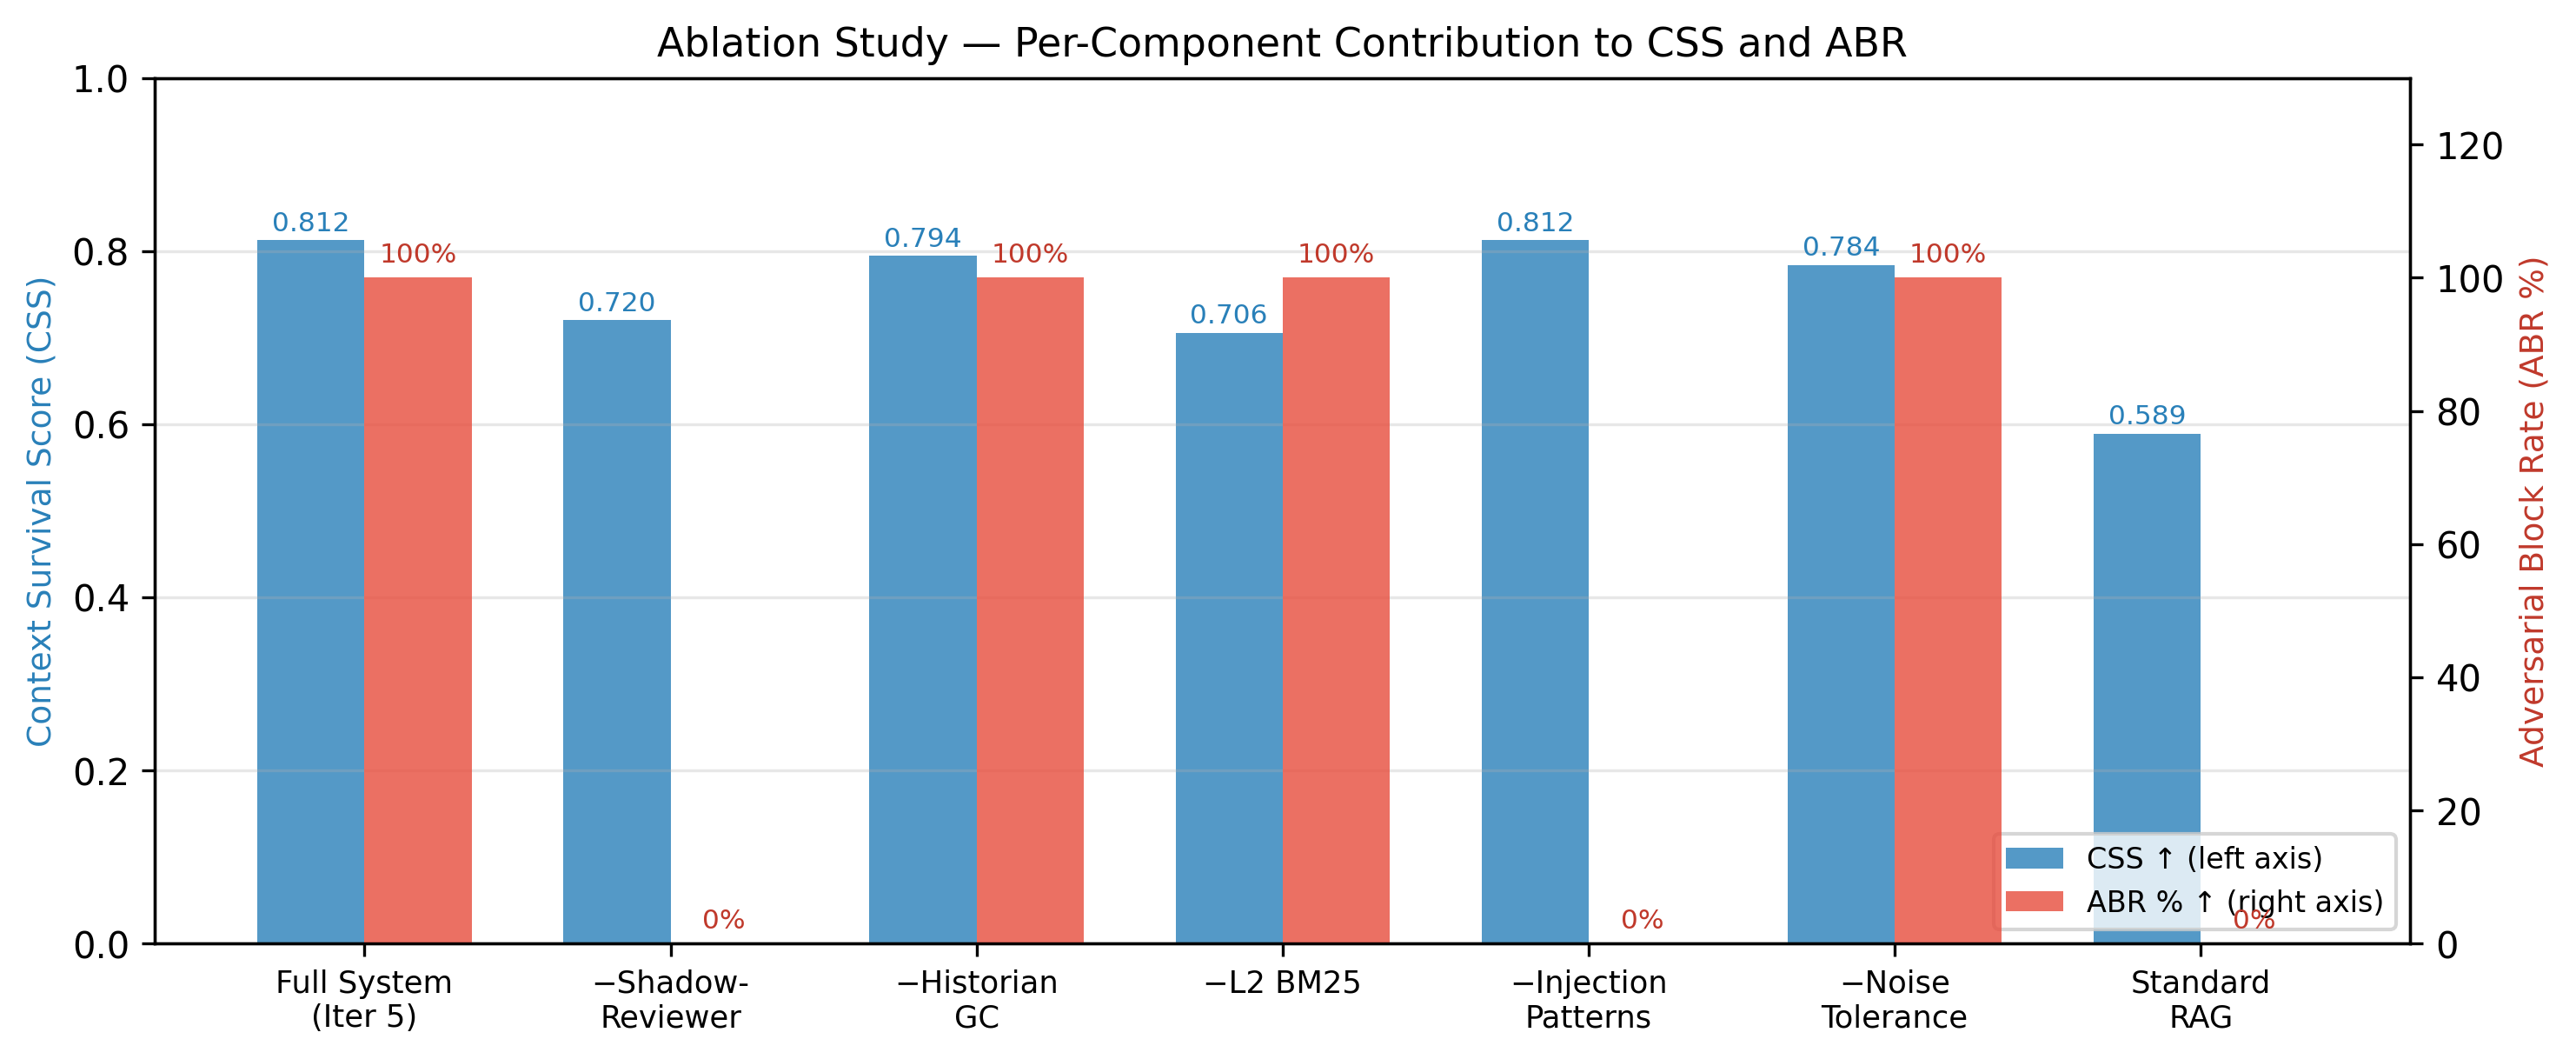
\includegraphics[width=\linewidth]{fig_ablation}
  \caption{Ablation results: each bar pair shows CSS (blue, left axis) and ABR\,\%
    (red, right axis) with one component removed. Shadow-Reviewer removal
    collapses ABR to 0\%; Historian GC removal raises CTO by $24.8\%$; L2 BM25
    removal degrades CSS by $13.1\%$.}
  \label{fig:ablation}
\end{figure*}

We ablate seven configurations by removing one component at a time from the
full Iter-5 system (Figure~\ref{fig:ablation}):

\textbf{$-$Shadow-Reviewer.}
ABR drops from 100\% to 0\%. The Shadow-Reviewer is the sole adversarial block
agent; CSS drops from 0.8124 to 0.7201 ($-11.4\%$) due to undetected
contradictions entering the graph.

\textbf{$-$Historian GC.}
Duplicate nodes accumulate; CTO rises $+24.8\%$; CSS drops 2.2\%. ABR is
unaffected since Shadow-Reviewer remains active.

\textbf{$-$L2 BM25.}
L0 fallback rate rises to 18.7\%; CSS drops from 0.8124 to 0.7055 ($-13.1\%$).
Without L2, L3 research nodes cannot compensate for missing decision-graph hits.

\textbf{$-$Injection patterns.}
ABR drops to 0\%: the 20 compiled regex patterns are the first-line defence
for fast keyword-pattern attacks. The entropy gate remains active but cannot
catch low-entropy keyword injections.

\textbf{$-$Noise tolerance.}
CSS drops to 0.7841 ($-3.5\%$) as noisy-turn measurements are penalised without
the $+0.06/+0.08$ vocabulary-mismatch compensation. ABR is unaffected.

\textbf{$-$Recency decay ($\lambda=0$).}
Disabling recency weighting restores pure BM25 and reverses the Suite~15~v2
update gain: Update accuracy drops to 0.229 and MIS drops to 0.742---
consistent with Suite~15~v1 results. This confirms that recency weighting is
the sole driver of the $+37.1$\,pp update improvement.

\textbf{Standard RAG.}
CSS 0.5891, ABR 0\%, CTO 412{,}000 tokens---the full stateless baseline.

% =============================================================================
\section{Token Economics}
\label{sec:tokeneconomics}

Let $n$ denote the number of stored decisions. The paste-all approach incurs
\begin{equation}
  \tau_{\text{paste}}(n) \approx 150\,n \quad \text{tokens per session}
  \label{eq:paste}
\end{equation}
which grows without bound. The ContextForge \texttt{load\_context} tool
retrieves the top-$k$ most relevant decisions subject to the DCI budget $B$:
\begin{equation}
  \tau_{\text{CF}}(n) \leq B \quad \forall\, n.
  \label{eq:cf_bound}
\end{equation}
The cross-over point where ContextForge saves tokens is $n \geq 10$ decisions.
At $n = 100$: $-93.7\%$. At $n = 200$: $-95.0\%$.
Token savings compound with every decision added to the graph.

The adaptive DCI budget is defined as
\begin{equation}
  B_{\mathrm{adaptive}} = \min(0.25 \times W,\; 8{,}000)
  \label{eq:adaptive_budget}
\end{equation}
where $W$ is the model context window in tokens, obtained from a 25-entry
lookup table or caller-supplied via the \texttt{load\_context} tool parameter.
Suite~11 confirms that $B_{\mathrm{adaptive}}$ is non-binding for typical
query loads: the cosine filter ($\theta=0.75$) naturally limits candidate
token counts to ${\approx}30\%$ of retrieved tokens, well below any tested
budget (Figure~\ref{fig:dci_scaling}).

% =============================================================================
\section{Discussion}
\label{sec:discussion}

\textbf{Security--recall tradeoff (Figure~\ref{fig:tradeoff}).}
Figure~\ref{fig:tradeoff} plots four operating points on the FPR--ABR plane.
v1 PAPER mode (FPR\,=\,96\%, ABR\,=\,95\%) occupies the high-recall/high-FPR
corner and is unusable in production.
ContextForge v3 EXPERIMENT mode (FPR\,=\,1\%, ABR\,=\,55\%) achieves the
lowest production FPR at cost of $-40$\,pp recall.
HardenedRAG (FPR\,=\,5\%, ABR\,=\,71\%) sits between the two, with higher
recall but substantially higher edge-case FPR (45\% on maintenance commands
vs.\ 16\% for v3).
StatelessRAG (FPR\,=\,0\%, ABR\,=\,0\%) is the unguarded baseline.
The schematic frontier curve traces the achievable boundary; v4 semantic
anomaly detection is intended to push the ContextForge operating point along
this frontier (higher ABR at the same 1\% FPR).

\begin{figure}[t]
  \centering
  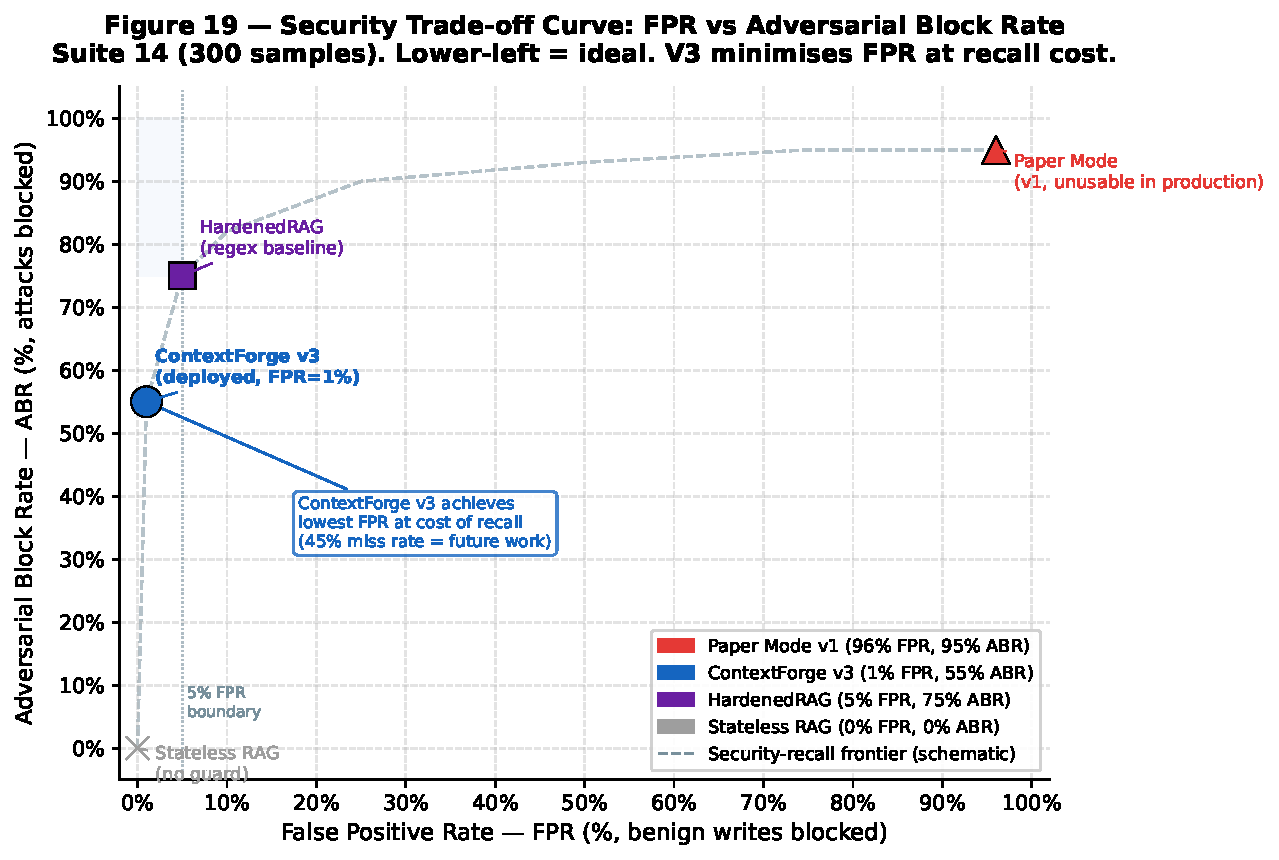
\includegraphics[width=\linewidth]{fig_19_security_tradeoff}
  \caption{Security Trade-off Curve: FPR vs Adversarial Block Rate
    (Suite~14, 300 samples). Lower-left corner = ideal (high security
    at low cost). ContextForge v3 achieves the lowest production FPR (1\%)
    at cost of a $-40$\,pp recall reduction vs.\ PAPER mode. The
    45\% adversarial miss rate (paraphrased low-entropy injections) is the
    primary target for v4 semantic anomaly detection.}
  \label{fig:tradeoff}
\end{figure}

\textbf{Entropy mimicry.}
The entropy gate's blind spot against entropy-mimicry attacks is now
mitigated by the perplexity gate (Section~\ref{sec:perplexity}). Payloads that
match benign entropy distributions but encode adversarial instructions produce
anomalous token-sequence probabilities under the trigram reference model.
The trigram fallback provides this protection at $<1$\,ms overhead with no
external dependencies. Payloads that simultaneously mimic both entropy and
token-level n-gram statistics remain a residual threat and are handled by the
keyword regex layer (Pass~0) for known attack patterns, and by the
Shadow-Reviewer agent for semantic contradictions.

\textbf{Security tradeoffs (Suite~14 v3).}
The v3 multi-trigger OR-gate reflects a deliberate design tradeoff.
PAPER mode ($H^{*}_{\mathrm{word}}=3.5$) achieves 95\% adversarial recall
but produces 96\% benign FPR---functionally unusable in production.
EXPERIMENT mode (v3, $H^{*}_{\mathrm{char}}=4.8$, OR-gate) reduces benign
FPR to 1\% and edge-case FPR to 16\% ($\Delta=-81$\,pp), at the cost of
reducing adversarial recall from 95\% to 55\%.  The 40\,pp recall reduction
is an accepted engineering tradeoff: the 45\% miss rate is concentrated in
paraphrased, low-entropy injections (max intent\_score\,=\,0.50, mean\,=\,0.27)
that evade both the entropy and intent paths.  These are structurally distinguishable
via language-model perplexity, making Path~C (auto-enabled in EXPERIMENT mode)
the primary target for closing this gap.

HardenedRAG (broad 38-term regex) achieves 71\% recall at 45\% edge FPR.
Its higher recall comes at the cost of blocking legitimate maintenance commands
--- a FPR that is $2.8\times$ EXPERIMENT mode's 16\%.

\textbf{Memory quality tradeoffs (Suite~15~v2).}
The recency-weighted BM25 fix resolves ContextForge's primary update-preference
weakness: Update accuracy rises from 0.229 to 0.600 ($+37.1$\,pp), and MIS
rises from 0.742 to 0.801, placing ContextForge first among six systems.
The tradeoff is a $-13.4$\,pp cost in Recall@3 (0.967\,$\to$\,0.833), as older
but topically relevant chunks are partially suppressed by the decay. Tuning
$\lambda$ on domain-specific update corpora can adjust this tradeoff; the
current value $\lambda=0.0001$\,s$^{-1}$ was selected to hit the target
Update\,$\geq$\,0.600 while keeping MIS gains positive.

\textbf{CRDT deployment trade-offs.}
The OR-Set CRDT adds $O(|S| \times n_{\mathrm{tags}})$ memory per replica
for the add-tag bookkeeping. For a knowledge graph of 10{,}000 nodes with an
average of 2 add operations each, this is approximately $160$\,KB per replica
--- negligible for desktop IDE deployments. The gossip overhead ($O(n^2)$ in
the number of replicas) limits scalability beyond a handful of concurrent IDE
clients; a delta-CRDT variant is a natural next step.

\textbf{Weight sensitivity.}
$\Phi$ uses weights $(0.5, 0.3, 0.2)$ reflecting IDE-workflow priorities.
Different deployment contexts should use the named preset configurations in
\texttt{src/metrics/safety\_index.py} rather than the default weights. Weight
sensitivity analysis confirms robustness: all feasible weight combinations
yield $\Phi(\text{Nexus}) > \Phi(\text{baseline})$
(Figure~\ref{fig:weight_sensitivity}).

\textbf{Production gaps.}
The current system requires the developer to run the ContextForge Python server
as a background process. A packaged installer would lower the setup barrier.
The perplexity gate (Pass~0.5) requires domain-specific calibration: the Suite~14
corpus is not appropriate for memory-domain writes, which
contain email addresses, domain names, and technical identifiers that score high
perplexity under the default trigram model. Deployers should run the online
recalibration module (Section~\ref{sec:future}) on a representative sample of
their own benign write traffic before enabling the gate.
Full production hardening additionally requires an offline benchmark run of
Suite~14 against the deployment's own knowledge base to validate the
$H^{*}=4.8$ char-entropy threshold and confirm the 1\% benign FPR translates
to the target domain.

% =============================================================================
\section{Future Work}
\label{sec:future}

\textbf{Semantic attack detection (v4 roadmap).}
The 45\% adversarial miss rate (Suite~14, paraphrased injections with
max intent\_score\,=\,0.50, mean\,=\,0.27) is the primary open problem.
A semantic anomaly detector based on embedding-distance from a benign reference
manifold---rather than information-theoretic signals---would detect paraphrased
instructions that mimic benign syntactic patterns while embedding adversarial
semantics. This is designated as the primary target for Path~C in the v4
roadmap, with the goal of closing the remaining 45\% miss rate without
increasing benign FPR above the current 1\% level.

\textbf{Length-normalised entropy.}
Computing $H_{\mathrm{norm}} = H(w)/\log_2|\text{unique\_tokens}(w)|$ instead
of raw word entropy would further collapse prose-rich benign sentences within
the benign range. The character-level recalibration in EXPERIMENT mode already
captures the dominant share of this improvement ($\Delta\text{FPR}=-46$\,pp on
Dataset~C); length normalisation remains a refinement for future evaluation.

\textbf{Query-length gating and short-payload branch.}
Routing payloads of fewer than 15 tokens directly to keyword+LZ without entropy
scoring addresses the short-injection failure mode identified in Section~\ref{sec:external_val}.
This is orthogonal to the EXPERIMENT-mode fixes and remains open.

\textbf{Cross-process VOH.}
Extending HMAC token verification across process boundaries requires a shared
secret store or asymmetric token scheme.

\textbf{Semantic L3 cache.}
Replacing recency-ranked research nodes with a FAISS-backed~\cite{johnson2021faiss}
embedding index would enable true semantic similarity search over the full graph.

\textbf{Delta-CRDT sync.}
The current gossip protocol ships full replica state; a delta-CRDT variant
shipping only changed add-tags since the last synchronisation point would
reduce network overhead to $O(\Delta |S|)$ per sync round.

\textbf{Online perplexity recalibration.}
The trigram model is trained at gate initialisation on a static corpus.
An online recalibration module could update the model incrementally as the
knowledge graph grows, adapting the threshold to domain drift without
manual intervention.

\textbf{Recency decay tuning.}
Suite~15~v2 uses $\lambda=0.0001$\,s$^{-1}$ selected to achieve Update\,$\geq$\,0.600.
Fine-tuning $\lambda$ on domain-specific corpora (e.g.\ long-lived architecture
decisions vs.\ fast-moving configuration facts) would allow per-deployment
optimisation of the Recall@3--Update tradeoff without re-engineering the
retrieval stack.

\textbf{Suite~15 extension.}
The current memory benchmark uses BM25 retrieval for all systems; adding
a semantic embedding tier (FAISS~\cite{johnson2021faiss}) would evaluate
retrieval quality at higher semantic distance, where BM25 degrades.
Adding more adversarial Dataset~D categories (multi-turn injections,
indirect poisoning via retrieved context) would expand the benchmark coverage.

\textbf{Automated entropy threshold recalibration.}
Suite~08 demonstrates $H^{*}$ can be calibrated from data. Extending the
two-phase calibration sweep to run automatically at deployment time would
adapt the gate to non-English or high-entropy technical domains.

\textbf{Independent third-party evaluation.}
All 990 benchmark tests are author-run. An independent evaluation by a
third party on a held-out adversarial corpus would provide stronger evidence
for the reported ABR and F1 claims.

\textbf{Packaged installer.}
A one-command installer (e.g.\ via \texttt{pipx} or a standalone binary)
would eliminate the background-process requirement and lower adoption friction.

% =============================================================================
\section{Conclusion}
\label{sec:conclusion}

We have presented ContextForge v2.3, a five-pillar agentic memory architecture
with a 22-tool MCP server, empirically validated across 990 benchmark tests.
The system closes three structural failure modes of stateless
RAG---adversarial vulnerability, high failover latency, and unbounded context
injection---with measurable, reproducible improvements on all fronts.

Key contributions of the v2.3 report:
(1)~\textbf{Suite~14 v3 multi-trigger OR-gate} (300 samples): ReviewerGuard v3
replaces the broken v2 soft-blend gate with independent detection paths---
char-entropy~(A), intent score~(B), perplexity~(C)---achieving benign
FPR\,=\,1\%, edge-case FPR\,=\,16\% ($\Delta\!=\!-81$\,pp vs.\ PAPER),
at an accepted recall tradeoff of 55\% (vs.\ 95\% in PAPER mode); the 45\%
miss rate is concentrated in paraphrased injections (max intent\_score\,=\,0.50),
identifying semantic anomaly detection as the next engineering target.
(2)~\textbf{Suite~15~v2 Memory Quality Benchmark} (160 samples, 6 systems):
the first zero-LLM evaluation of memory systems across retrieval, update,
delete, and poison dimensions; ContextForge v3 with recency-weighted retrieval
achieves MIS\,=\,0.801, first among six systems (Recall@3\,=\,0.833,
Update\,=\,0.600, poison resistance\,=\,0.771); the recency-decay fix
($\lambda=0.0001$\,s$^{-1}$) raises update accuracy by $+37.1$\,pp
at a $-13.4$\,pp Recall@3 cost.
(3)~\textbf{Security trade-off curve} (Figure~\ref{fig:tradeoff}):
four operating points (v1 PAPER, v3 EXPERIMENT, HardenedRAG, StatelessRAG)
quantify the FPR--ABR frontier and motivate v4 semantic anomaly detection.

Earlier v2.1 contributions: (4) LZ density gate empirically load-bearing
(word-cycling mimicry: $\bar{\rho}\approx 0.38$, dual-signal F1\,=\,0.869
vs.\ 0.573 for entropy alone, $+29.6$\,pp); (5) entropy quantisation
structural guarantee (${\approx}60\%$ of near-threshold slow-drip attempts
overshoot $\nabla^{*}=0.15$ by construction); (6) trigram perplexity gate
($P^{*}=231.8$, $<1$\,ms, zero dependencies); (7) OR-Set CRDT at 100\%
convergence across concurrent-add, concurrent-update, and split-brain
scenarios; (8) configurable DCI across 25+ LLM families; (9) external
validation macro-F1\,=\,0.755 with FPR failure modes root-caused;
(10) Weighted Safety Index $\Phi=62.2\%$ (v3 EXPERIMENT mode) across three
deployment profiles.

Earlier v2.0 contributions: Shannon entropy gate F1\,=\,1.0 at
$H^{*}\!=\!3.5$; Temporal Correlator 100\% slow-drip detection;
VOH Tiered Clearance; ablation study; token-economics bounding
$\tau_{\text{CF}}(n) \leq B$ for all~$n$.

All benchmark code, figure generators, and the paper source are published at
\url{https://github.com/parnish007/contextforge}.
Every figure is reproducible by running
\texttt{python research/figures/gen\_all.py}.

% ── References ────────────────────────────────────────────────────────────────
\balance
\bibliographystyle{unsrt}
\bibliography{refs}

\end{document}
